% ==============================================================
% File     : main.tex
% Date     : 26 Nov. 2021
% Revision : 30 July 2022
% Creator  : Marco Peressutti
% ==============================================================

\documentclass[a4paper, 10pt, oneside]{book}
\usepackage[utf8]{inputenc}
 

% ==============================================================
% File     : lib/includes.tex
% Date     : 26 Nov. 2021
% Revision : 30 July 2022
% Creator  : Marco Peressutti
% ==============================================================

% ==============================================================
% $package-name$ : type     : $description$
% --------------------------------------------------------------
% amsmath        : math     : AMS mathematical facilities for LaTeX
% amssymb        : math     : AMS symbols
% amsthm         : math     : Typesetting theorems (AMS style)

% babel          : biblio   : Multilingual suppor for latex ...
% biblatex       : biblio   : Sophisticated Bibliographies in LaTeX
% bm             : math     : Access bold symbols in maths mode
% booktabs       : tables   : Publication quality tables in LaTeX

% cancel         : math     : Place lines through maths formulae
% csquotes       : misc     : Context sensitive quotation facilities

% dirtytalk      : misc     : A package to typeset quotations easier

% empheq         : math     : EMPHasizing EQuations
% enumitem       : misc     : Control layout of itemize, enumerate, description

% fancyhdr       : page     : Extensive control of page headers and footers in LaTeX2epsilon
% fontenc        : font     : Standard package for selecting font encodings

% geometry       : page     : Flexible and complete interface to document dimensions
% glossaries     : misc     : Create glossaries and lists of acronym
% graphicx       : graphics : Enhanced suppoort for graphics

% hyperref       : misc     : Extensive support for hypertext in LaTeX

% listings       : code     : Typeset source code listings using LaTeX
% lmodern        : font     : Latin modern fonts in outline formats

% makecell       : misc     : Tabular column heads and multilined cell
% marginnote     : page     : Notes in the margin, even where \marginpar fails
% mathtools      : math     : Mathematical tools to use with amsmath
% microtype      : font     : Subliminal refinements towards typographical perfection
% minitoc        : misc     : Produce a table of contents for each chapter, part or section

% nicematrix     : math     : Improve the typesetting of mathematical matrices with PGF

% pifont         : font     : Access to PostScript standard Symbol and Dingbats fonts

% setspace       : misc     : Set space between lines
% subcaption     : graphics : Support for sub-captions

% tabularx       : tables   : Tabulars with adjustable-width columns
% todonotes      : page     : Marking things to do in a LaTeX document

% xcolor         : misc     : Driver-independent color extensions for LaTeX and pdfLaTeX
% xfrac          : math     : Split-level fractions in LaTeX2epsilon
% ==============================================================

\usepackage[right=30.2mm, left=28.4mm, marginparwidth=75pt, top=20mm]{geometry}
%\usepackage[a4paper, marginparwidth=75pt, total={10cm, 10cm}]{geometry}

\usepackage[english]{babel} 
\usepackage[bibstyle=numeric, backend=biber, sorting=nty]{biblatex}

\usepackage{listings}

\usepackage[T1]{fontenc}    
\usepackage{lmodern}        
\usepackage{microtype}      
\usepackage{pifont}

\usepackage{graphicx}       
\usepackage{subcaption}

\usepackage{amsmath} 
\usepackage{amssymb} 
\usepackage{mathtools} 
\usepackage{amsthm}
\usepackage[makeroom]{cancel}
\usepackage{empheq}
\usepackage{nicematrix}
\usepackage{xfrac}
\usepackage{bm}

\usepackage{tabularx}
\usepackage{booktabs}
%\usepackage{minitoc}

\usepackage{marginnote}
\usepackage{todonotes}
\usepackage{fancyhdr}

\usepackage{dirtytalk}      
\usepackage{csquotes}
\usepackage[acronym, nonumberlist, seeautonumberlist]{glossaries}
\usepackage{hyperref}
\usepackage{setspace}
\usepackage{enumitem}
\usepackage{xcolor}
\usepackage{makecell}

\usepackage[most,many,breakable]{tcolorbox}

\usepackage{titlesec, titletoc} %// TODO: add these to the description above
\usepackage{algorithm, algorithmic} % usepackages
% ==============================================================
% File     : lib/acronyms.tex
% Date     : 30 July 2022
% Revision : 30 July 2022
% Creator  : Marco Peressutti
% ==============================================================

\newacronym{HW}{HW}{Hardware}
\newacronym{SW}{SW}{Software}
\newacronym{OS}{OS}{Operating System}
\newacronym{RTOS}{RTOS}{Real-Time Operating System}
\newacronym{RM}{RM}{Rate Monotonic}
\newacronym{DM}{DM}{Deadline Monotonic}
\newacronym{EDF}{EDF}{Earliest Deadline First}
\newacronym{IPC}{IPC}{Inter-Process Communication}
\newacronym{I/O}{I/O}{Input/Ouput} % acromyms
% ==============================================================
% File     : lib/commands.tex
% Date     : 26 Nov. 2021
% Revision : 30 July 2022
% Creator  : Marco Peressutti
% ==============================================================

\defbibheading{bibempty}{}
% ==============================================================
% NEW-COMMANDS:
% ==============================================================

% \M         : matrix with square    delimiters/brackets
% \B         : matrix with curly     delimiters/brackets
% \und       : underline math expression in math mode
% \pd        : (first  order) partial derivative
% \td        : (first  order) total   derivative
% \pdd       : (second order) partial derivative 
% \tdd       : (second order) total   derivative
% \omissis   : three dots surrounded by square brackets
% \pexp      : pre exponent (#1) of symbol (#2) where \pexp{#1}{#2} 
% \ret       : left arrow symbol as exponent 
% \smalltodo : [internal] DO NOT USE 
% \side      : size notes (yellow line to the side of the page with text)
% \pside     : phantom side (used in environment where the \side causes compilation errors)
% \ceil      : ceil  brackets
% \floor     : floor brackets 
% \degr      : degree symbol (just an exponent with circle in front of the number)

\newcommand{\M}[1]{\begin{bmatrix}#1\end{bmatrix}}
\newcommand{\und}[1]{\underline{#1}}
\newcommand{\B}[1]{\begin{Bmatrix}#1\end{Bmatrix}}
\newcommand{\pd}[2]{\cfrac{\partial#1}{\partial#2}}
\newcommand{\td}[2]{\cfrac{d#1}{d#2}}
\newcommand{\pdd}[2]{\cfrac{\partial^2#1}{\partial#2^2}}
\newcommand{\tdd}[2]{\cfrac{d^2#1}{d#2^2}}
\newcommand{\omissis}{[\textellipsis\unkern]}
\newcommand{\pexp}[2]{\prescript{#1}{}{#2}{}{}}
\newcommand{\ret}[1]{{#1}^{\leftarrow}}
\newcommand{\smalltodo}[2][]{\todo[caption={#2}, #1, backgroundcolor=white!20!white, bordercolor=white]{\begin{spacing}{0.5}\texttt{#2}\end{spacing}}}
\newcommand{\side}[1]{\smalltodo[size=\footnotesize]{#1}\textbf{#1}}
\newcommand{\pside}[1]{\smalltodo[size=\footnotesize]{#1}}
\newcommand{\ceil}[1]{\left\lceil #1 \right\rceil}
\newcommand{\floor}[1]{\left\lfloor #1 \right\rfloor}
\newcommand{\degr}[1]{^{\circ\!#1}}

% ==============================================================
% RE-NEW-COMMANDS:
% ==============================================================

% prettier \theta symbol
\renewcommand{\theta}{\vartheta}
% prettier \epsilon symbol
\renewcommand{\epsilon}{\varepsilon}
% I have no clue what \arraystretch does prolly used internally in itemize/enumerate environment
\renewcommand{\arraystretch}{1.3}

% ==============================================================
% DECLARES:
% ==============================================================

% \abs      : absolute value operator/delimiters (i.e. |  expression  |)
% \norma    : norm           operator/delimiters (i.e. || expression ||)
% \minimize : "minimize" that allows to write things just under the symbol 
% \argmin   : "argmin" that allows to write things just under the symbol
\DeclarePairedDelimiter\abs{\lvert}{\rvert}
\DeclarePairedDelimiter{\norma}{\lVert}{\rVert}
\DeclareMathOperator*{\minimize}{minimize}
\DeclareMathOperator*{\argmin}{argmin}


% ==============================================================
% MISC:
% ==============================================================

% more compact representtation of itemize
\setitemize{noitemsep,topsep=10pt,parsep=0pt,partopsep=0pt}

% colors
\definecolor{codegreen}{rgb}{0,0.6,0}
\definecolor{codegray}{rgb}{0.5,0.5,0.5}
\definecolor{codepurple}{rgb}{0.58,0,0.82}
\definecolor{backcolour}{rgb}{0.95,0.95,0.92}
\definecolor{myb}{RGB}{45, 111, 177}
\definecolor{myr}{RGB}{199, 68, 64}
\definecolor{myg}{RGB}{90, 199, 90}

% Code snippets style
\lstdefinestyle{mystyle}{
    backgroundcolor=\color{backcolour},   
    commentstyle=\color{codegreen},
    keywordstyle=\color{magenta},
    numberstyle=\tiny\color{codegray},
    stringstyle=\color{codepurple},
    basicstyle=\ttfamily\footnotesize,
    breakatwhitespace=false,         
    breaklines=true,                 
    captionpos=b,                    
    keepspaces=true,                 
    numbers=left,                    
    numbersep=5pt,                  
    showspaces=false,                
    showstringspaces=false,
    showtabs=false,                  
    tabsize=2
}
\lstset{style=mystyle}

\makeatletter
\newcommand\incircbin
{%
  \mathpalette\@incircbin
}
\newcommand\@incircbin[2]
{%
  \mathbin%
  {%
    \ooalign{\hidewidth$#1#2$\hidewidth\crcr$#1\bigcirc$}%
  }%
}
\newcommand{\ooplus}{\incircbin{+}}     % A circle with a plus  inside
\newcommand{\oominus}{\incircbin{-}}    % A circle with a minus inside
\newcommand{\oocirca}{\incircbin{\sim}} % A circle with a tilde inside
\makeatother

\newcommand{\cmark}{\ding{51}} % literally a  tick
\newcommand{\xmark}{\ding{55}} % literally an X

% equal with symbol on top
\newcommand\equal[1]{\stackrel{\mathclap{\footnotesize\mbox{#1}}}{=}}

% text without double lined line
\newcommand{\textbetweendoublerules}[2][.4pt]{%
  \par\addvspace{\topsep}
  \noindent\makebox[\textwidth]{%
    \sbox0{\quad#2\quad}%
    \dimen0=.5\dimexpr\ht0+#1\relax
    \dimen2=-.5\dimexpr\ht0-#1\relax
    \dimen4=.5\dimexpr\textwidth-\wd0\relax
    \setbox2=\vbox to \ht0{%
      \vss
      \hrule width \dimen4 height #1
      \kern 4\dimexpr#1\relax
      \hrule width \dimen4 height #1
      \vss
    }%
    \copy2 \box0 \box2
  }\par\nopagebreak\addvspace{\topsep}%
}


% red box used for examples
\makeatletter
\newtcbtheorem{iexample}{Example}{enhanced,
	breakable,
	colback=white,
	colframe=myr!80!black,
	attach boxed title to top left={yshift*=-\tcboxedtitleheight},
	fonttitle=\bfseries,
	title={#2},
	boxed title size=title,
	boxed title style={%
			sharp corners,
			rounded corners=northwest,
			colback=tcbcolframe,
			boxrule=0pt,
		},
	underlay boxed title={%
			\path[fill=tcbcolframe] (title.south west)--(title.south east)
			to[out=0, in=180] ([xshift=5mm]title.east)--
			(title.center-|frame.east)
			[rounded corners=\kvtcb@arc] |-
			(frame.north) -| cycle;
		},
	#1
}{def}
\makeatother

% blue box used for definitions
\makeatletter
\newtcbtheorem{idefinition}{Definition}{enhanced,
	breakable,
	colback=white,
	colframe=myb!80!black,
	attach boxed title to top left={yshift*=-\tcboxedtitleheight},
	fonttitle=\bfseries,
	title={#2},
	boxed title size=title,
	boxed title style={%
			sharp corners,
			rounded corners=northwest,
			colback=tcbcolframe,
			boxrule=0pt,
		},
	underlay boxed title={%
			\path[fill=tcbcolframe] (title.south west)--(title.south east)
			to[out=0, in=180] ([xshift=5mm]title.east)--
			(title.center-|frame.east)
			[rounded corners=\kvtcb@arc] |-
			(frame.north) -| cycle;
		},
	#1
}{def}
\makeatother

% green box used for theorems
\makeatletter
\newtcbtheorem{itheorem}{Theorem}{enhanced,
	breakable,
	colback=white,
	colframe=myg!80!black,
	attach boxed title to top left={yshift*=-\tcboxedtitleheight},
	fonttitle=\bfseries,
	title={#2},
	boxed title size=title,
	boxed title style={%
			sharp corners,
			rounded corners=northwest,
			colback=tcbcolframe,
			boxrule=0pt,
		},
	underlay boxed title={%
			\path[fill=tcbcolframe] (title.south west)--(title.south east)
			to[out=0, in=180] ([xshift=5mm]title.east)--
			(title.center-|frame.east)
			[rounded corners=\kvtcb@arc] |-
			(frame.north) -| cycle;
		},
	#1
}{def}
\makeatother


% green box used for theorems
\makeatletter
\newtcbtheorem{ilemma}{Lemma}{enhanced,
	breakable,
	colback=white,
	colframe=myg!80!black,
	attach boxed title to top left={yshift*=-\tcboxedtitleheight},
	fonttitle=\bfseries,
	title={#2},
	boxed title size=title,
	boxed title style={%
			sharp corners,
			rounded corners=northwest,
			colback=tcbcolframe,
			boxrule=0pt,
		},
	underlay boxed title={%
			\path[fill=tcbcolframe] (title.south west)--(title.south east)
			to[out=0, in=180] ([xshift=5mm]title.east)--
			(title.center-|frame.east)
			[rounded corners=\kvtcb@arc] |-
			(frame.north) -| cycle;
		},
	#1
}{def}
\makeatother


% command to use the definition box \definition{Name}{Verbose definition of Name}
\newcommand{\definition}[2]{\begin{idefinition}{#1}{}#2\end{idefinition}}
% command to use the definition box \definition{(optional) Example title}{Verbose description of Example}
\newcommand{\example}[2]{\begin{iexample}{#1}{}#2\end{iexample}}
% command to use the definition box \definition{(optional) Example title}{Verbose description of Example}
\newcommand{\theorem}[2]{\begin{itheorem}{#1}{}#2\end{itheorem}}
\newcommand{\lemma}[2]{\begin{ilemma}{#1}{}#2\end{ilemma}}

% used to make table of contents for each part
\titleclass{\part}{top}
\titleformat{\part}
  {\centering\normalfont\Huge\bfseries}{}{0pt}{}
\setcounter{secnumdepth}{5} % newcommands

% title page
\title{145071 - Real time operating systems\\ and middleware}
\author{Marco Peressutti\\230403\\marco.peressutti@studenti.unitn.it}
\date{\today}

% chapters
\includeonly{
  chapters/00-IntroductionToTheCourse,
  chapters/01-BasicConcepts,
  chapters/02-PeriodicTaskScheduling,
  chapters/03-AperiodicServers,
  chapters/04-ResourceAccessProtocols,
  chapters/05-TheKernel,
  chapters/06-TimerAndClockLatency,
  chapters/07-TheNonPreemptableSectionLatency,
  chapters/0A-UlubRM,
  chapters/0B-UlubRM-PS,
  chapters/0C-UlubRM-DS,
  chapters/Posix
}

% bibliography resources
\addbibresource{bib/bibliografia.bib}
% path to images
\graphicspath{{images/}}
% load acronyms
\makeglossaries

\begin{document}

    \selectlanguage{english}
    
    \maketitle
    \printglossary[type=\acronymtype]
    
    %% frontmatter
    \frontmatter
    \setcounter{page}{1}
    \cleardoublepage

    \fancypagestyle{plain}{}
    \renewcommand{\chaptermark}[1]{ \markboth{#1}{}} 
    \tableofcontents
      \markboth{\contentsname}{}      
    \cleardoublepage

    %% mainmatter
    \mainmatter
  
    \chapter*{Introduction to the Course}
\section*{Material}
\begin{itemize}
    \item Slides available from moodle
    \item Interested students can have a look at: \textit{Giorgio Buttazzo}, \textbf{HARD REAL-TIME COMPUTING SYSTEMS: Predictable Scheduling Algorithms and Applications}
\end{itemize}
\section*{Exam}
\subsection*{Written Exam}
\begin{itemize}
    \item 3 questions, 30 minutes per question
    \item Each answer gets a score from 0 to 30
    \item (Optional) project
\end{itemize}

\subsection*{Oral Exam}
\begin{itemize}
    \item Discussion of the written exam
    \item Open Questions or Discussion on a project
\end{itemize}

\section*{Prerequisites}
\begin{itemize}
    \item Programming skills: C, maybe C++.\\
    You must know how ot code in C (optionally C++). This is not about knowing the C syntax, it is about writing good and clean C code.\\
    To help overcome this lack of prerequisites please consider reading the book \textit{Kerrigan \& Ritchie},\textbf{The C Programming Language}
    \item Knowledge about Operating Systems.\\
    This prerequisites is met if you have taken the course \textit{Sistemi Operativi 1} or similar exams.\\
    Alternatively please refer to a good Operating Systems book (e.g. Stallings,\dots).\\
    This includes how to use a shell, basic POSIX commands, \texttt{make}, how to compile, \dots.
\end{itemize}

\section*{Overview of the Course}
The course will cover 6 main macro areas of real time operating systems and middleware.
\begin{enumerate}
    \item Real Time Systems:
    \begin{itemize}
        \item Real-Time Computing and temporal constraints.\\
        Real time systems are software and hardware systems (hence computing systems), that have to comply with temporal constraints.
        \item Definitions and task model\\
        We will make things much clearer and better defined by introducing a sequence of definitions and mathematical models that will allow us to given this notion of temporal constraint a well founded meaning.
        \item Real-Time Scheduling\\
        We will also study solutions that allow us to enforce these real time constraints and this solution will have much to do on how we schedule shared resources.
    \end{itemize}
    \item Real-Time programming, RT-POSIX, pthreads,\dots\\
    We will move to a concrete ground and see what is the exact shape that these notions take once they are moved in a computer program. 
    \item Real-Time Scheduling algorithms:
    \begin{itemize}
        \item Fixed Priority scheduling, RM, DM
        \item EDF and dynamic priorities
        \item Resource Sharing (Priority Inversion, \dots)
    \end{itemize}
    As regards the Real-Time scheduling we will see many interesting policies, but since this is not a course on Real Time scheduling what we will do is provide the knowledge of real time scheduling so that the reader will be able to understand the mechanism of real time operating systems and thereby make best use of these technologies in future projects.
    \item Operating System Structure
    \begin{itemize}
        \item Notes about traditional kernel structures\\
        In order to keep latencies in check, we need proper technological solutions that make our operating systems differ quite a bit from standard operating systems.
        \item Sources of kernel latencies
        \item Some approaches to real-time kernels (e.g. dual kernel approach, interrupt pipes, microkernels, monolithis kernels and RT)
    \end{itemize}
    \item Real-Time Kernels and OSs.
    \item Developing Real-Time applications
\end{enumerate}

\subsection*{Real-Time Operating Systems}
In order to discuss about the Real-Time systems we need to provide some basic definitions:
\definition{Real-Time Operating Systems (RTOS)}{Operating Systems that provide support to Real-Time Applications}
\definition{Real-Time application}{the correctness depends not only on the output values, but also on the time when such values are produced}
\definition{Operating Systems (OS)}{
    \begin{itemize}
        \item Set of computer programs, of critical programs to be precise: because they have to be written efficiently, otherwise the hardware resources get disrupted, hence the system cannot operate correctly.
        \item Interface between applications and hardware. 

        Whenever an application interacts with an hardware, it is not of the developer interest to directly control the hardware. The Operating System provides an API that enables you to open a connection to a peripheral and takes care of all the low level interactions.
        On this regard, understanding the notion of interrupt will be of fundamental importance, because it is, essentially, what gave rise to concurrent programming: in the case we would like to interact with a peripheral, rather than continuously check if the peripheral has ended what it is supposed to do, you can tell the peripheral to communicate when it has completed the given task.
        
        Anyway the Operating systems acts as an interface towards the hardware and hides away all these complex details.
        \item Control the execution of application programs
        \item Manage the hardware and software resources
    \end{itemize}
}

Since the Operating System is something that lies in-between the user application and the hardware resources we can summarize the aforementioned interpretation of 
\begin{itemize}
    \item \side{Service Provider} for user programs (i.e. exports a programming interface).
    
    This concept looks at the OS from the perspective of the software application, in the sense that the Operating Systems provides to the application a series of services:
        \begin{itemize}
        \item Process Synchronization mechanism
        \item Inter-Process Communication (IPC)
        \item Process/Thread Scheduling, i.e.  ways to create and schedule tasks
        \item Input/Output
        \item Virtual Memory
        \end{itemize}
    And all these services are accessible through an API.


    \item \side{Resource Manager}\\
    If you think at the Operating System as a Resource Manager, then it is something that takes care of many things:
    \begin{enumerate}
        \item \side{Process Management}\\
        The fact that multiple applications can run at the same time on a PC, even though there is a small amount of processor available to manage these applications. (generally 2,4 or 8).
        
        The number of application that you are likely to create is often on the hundreds, hence it is necessary to make an appropriate sharing of the limited resources that you have in order for all the applications to live correctly.
        \item \side{Memory Management}\\
        Supposing one is using a 64-bit architecture, what will happen is that a space of memory is addressable with 64 bit. As a consequence we can imagine that the addressable memory is space has $2^{64} - 1$ memory locations available.
        
        And each application sees, these much space available for its execution. But however large the space can be in a machine, it will never match the aforementioned size. It could potentially for one task, but in the case a machine is hundreds of tasks and each of them wants to use that much memory, there is no way that the hardware can provide enough physical memory to satisfy all of them.
        
        To counteract this problem, it is common practice to schedule the memory as well, because you take advantage of the fact that an application CAN use $2^{64} - 1$ memory locations, but at a given time it uses a tiny portion of these locations. It is only that tiny portion of memory locations that needs to be made available to the running task.
        
        In this scenario, the OS makes it possible to accommodate within the physical memory of the computer these small slices of the available space that the application uses. So somehow it operates as a resource manager for the memory as well.
        \item \side{File Management}
        \item \side{Networking}, \side{Device Drivers}, \side{Graphical Interface}
        \end{enumerate}
        The important thing is that all of these resources, like the processor, the memory, the drivers etc..., are shared between all the tasks.
        All these resource managers have to be distributed among all the spectrum of tasks in such a way that the tasks behave properly, i.e. if you do not provide frequently enough these resources they would not be able to deliver the result on time (the OS manages this problem on its own).
        
        In the case we decide to look at the Operating System as a Resource Manager, we need to think of a structure for the OS that makes this resource management effective, effective in the sense that we believe it is the most relevant for our specific range of application.
        
        The way OSs handles devices, interrupt, etc. can be very different (and optimized in very different ways) depending on the type of application one is looking at. However, the type of optimizations we are interested in are those that allow our application to have time-limited execution.
\end{itemize}



\subsection*{Real-Time Systems}
A \side{Real-Time application} is an application of which the time when a result is produced matters.

In particular:
\begin{itemize}
\item a correct result produced too late is equivalent to a wrong result, or to no result.
\item it is characterized by temporal constraints that have to be respected.
\end{itemize}

\example{Mobile vehicle}{
    Let us consider a mobile vehicle with a software module that
    \begin{enumerate}
        \item Detects obstacles
        \item Computes a new trajectory to avoid them
        \item Computes the commands for engine, brakes,\dots
        \item Sends the commands
    \end{enumerate}
    If you decide to steer to the left or to the right there is a limited amount of time in which the operation has to be carried out. Hence if one can find an extremely effective strategy for steering the wheels but the strategy amounts to setting the values for the motors after one second, it is completely useless, since the vehicle is most likely to crash.

Hence a time violation in executing a task is a critical problem: it means that the developed application is useless and also dangerous.

But then, what is a reasonable time frame for completing the steering operation?\\
Depends on the speed in which the vehicle is traveling. But no matters if the vehicle is traveling at high or low speed the timing constraint is there, and if it is violated, the vehicle will eventually crash against the obstacle.

As a consequence: when a constraint is set, that constraint needs to be respected. And this is one of the core concept of Real Time.
}

Hence, a Real-Time is not necessarily synonym of fast execution, but rather of \side{predictable} execution.\\
Real time computing has much more to do with predictability than of being quick.


Some examples of temporal contraints are:
\begin{itemize}
    \item The program must react to external events in a predictable time
    \item The program must repeat a given activity at a precise rate
    \item The program must end an activity before a specified time
\end{itemize}

In this case, we can clearly notice that the temporal constraints can be either one shot events or periodic events, but in both cases, a common characteristic, there is a need of being predictability.\\
Temporal constraints are modeled using the concept of \side{deadline}.


Please notice that a Real-Time system is not just a \textit{fast system}, because the speed is always relative to a specific environment, i.e. the steering commands temporal constraint is set by the velocity of the vehicle.

Running faster is good, but does not guarantee the correct behavior. In fact, it is far more valuable to that temporal constraints are always respected; in other terms Real time systems prefer to run fast enough to respect the deadlines, to be reliable.

Hence, the type of analysis that is necessary to perform is not an analysis based on of average/typical cases but rather an analysis of worst case: I have to prove that even in the worst-case scenario, there is not deadline violation.

This predictability creates a wide gap between what a Real Time system is and what a general purpose system is, because general purpose systems are optimised for the average case, but a real time system only cares about the worst case. As a consequence, the way one designs a Real Time system is very different from the way a general purpose system is designed.\\
In fact:
\begin{itemize}
\item When one optimize for the average case, what one would look at is the number of times that an application completes a task every second, and this is called \side{Throughput}.
\item When one have a worst case requirement, the notion of throughput is not relevant anymore, and the analysis focuses in every single instance the maximum delay will be bounded.
\end{itemize}

Let us introduce some notion and general terms that we will extensively using during the course
\definition{Algorithm}{Logical procedure used to solve a problem}
\definition{Program}{Formal description of an algorithm, using a \textit{programming language}}
\definition{Process}{Instance of a program (program in execution)}
\definition{Thread}{Flow of execution, something that is able to execute using your processor along with other threads. These threads can be part of the same program and they can be executed in parallel.}
\definition{Task}{Process or thread}

Hence there are two different ways of sharing resources: one are threads in which your share computing resources and memory space, and processes in which you share computer resources but each of the processes has its own memory space.\\
Unfortunately, there is no common definition of a task: somebody use the terms with the same meaning as a thread and sometimes it is used with the same meaning as a process. In this class we will refer to threads.\\
Henceforth, when we talk about a task we will refer to a program that it is running and they share the same memory space with other programs.
    % exam, lab sessions
    % resources
    % what does real time means
    % achieving predictability

    \chapter{Basic Concepts}

A task can be seen as a sequence of actions and a deadline must be associated to each one of them.\\
We, therefore, are after is a definition of a formal model that identifies what these tasks or actions are and associate deadlines with them.

\section{Real-Time Tasks}
\definition{Real-Time Task ($\tau_i$)}{stream of jobs (or instances) $J_{i,k}$, or, in other terms, a sequence of activities that is activated periodically or aperiodically}

Each job $J_{i,k} =  (r_{i,k}, c_{i,k}, d_{i,k})$ is characterised by the following quantities:
\begin{itemize}
    \item{\makebox[1cm]{$r_{i,k}$\hfill}activation time}\pside{activation time}\\
    It is the time at which a task becomes ready for execution; it is also referred as \textit{request time} or \textit{release time}. 
    \item{\makebox[1cm]{$c_{i,k}$\hfill}computation time}\pside{computation time}\\
    Time necessary to the processor for executing the job without interruption.
    \item{\makebox[1cm]{$d_{i,k}$\hfill}absolute deadline}\pside{absolute deadline}\\
    time before which a job should be completed to avoid damage to the system.
    \item{\makebox[1cm]{$f_{i,k}$\hfill}finishing time}\pside{finishing time}\\
    The time at which a job finishes its execution
    \item{\makebox[1cm]{$\rho_{i,k}$\hfill}response time}\pside{response time}\\
    The time at which a job finishes its execution. Formally this quantity is the difference between the finishing time and the activation time.
    \[\rho_{i,k}  = f_{i,k} - r_{i,k}\]
\end{itemize}
Furthermore, since each task $i$ is a sequence of jobs, we need to differentiate between them. That is why each job $J_{i,k}$ is uniquely identified by its task index $i$ and the $k$-th activation of the $i$-th task.\\
In addition, we will say that job $J_{i,k}$ respects its deadline if $f_{i,k} \le d_{i,k}$.



\begin{figure}[!ht]
    \centering
    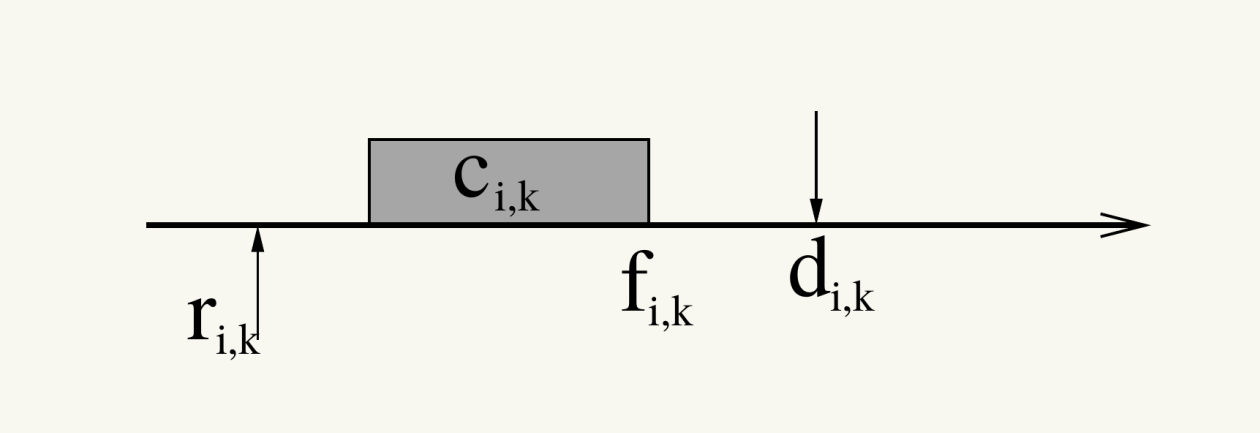
\includegraphics[width = 0.8\textwidth]{images/image01.png}
    \caption{Graphical representation of Mathematical model of a Task}
    \label{fig:image01}
\end{figure}

This mathematical definition of a job in a real-time task holds regardless of the nature of the task itself. In fact, we can identify three different types of tasks: Periodic tasks, Aperiodic Tasks and Sporadic Tasks.
Each of them holds different properties and a different mathematical representation.

\subsection{Periodic Tasks}

\definition{Periodic Task}{A periodic task $\tau_i = (C_i, D_i, T_i)$ is a stream of jobs $J_{i,k}$, with:
\begin{align*}
r_{i,k+1} &= r_{i,k} + T_i\\
d_{i,k} &= r_{i,k} + D_i\\
C_i &= \max_k\{c_{i,k}\}
\end{align*}
}
where:
\begin{itemize}
    \item{\makebox[1cm]{$T_i$\hfill}\textbf{Period}}\pside{Period}
    \item{\makebox[1cm]{$D_i$\hfill}\textbf{Relative Deadline}}\pside{Relative Deadline}
    \item{\makebox[1cm]{$C_i$\hfill}\textbf{Worst-Case Execution Time (WCET)}}\pside{Worst-Case Execution Time (WCET)}
    \item{\makebox[1cm]{$R_i$\hfill}\textbf{Worst-Case Response Time (WCRT)}}\pside{Worst-Case Response Time (WCRT)}
    \[R_i = \max_k \{\rho_{i,k}\}=\max_k \{f_{i,k} - r_{i,k}\}\]
\end{itemize}
For the task to be correctly scheduled, it must be $R_i \le D_i$

A periodic task has a regular structure (called \side{cycle}), in the sense that:
\begin{itemize}
\item it is activated periodically with a period of $T_i$
\item it executes a computation
\item when the computation terminates, it suspends waiting for the next period
\end{itemize}

Hence, its fundamental implementation can be represented as:
\begin{lstlisting}[language=C++]
void *PeriodicTask(void *arg)
{
	<initialization>;
	<start periodic timer, period = T>;
	while (condition)
	{
		<read sensors>;
		<update outputs>;
		<update state variables>;
		<wait next activation>;
	}
}
\end{lstlisting}

\subsection{Aperiodic Tasks}

\definition{Aperiodic Task}{Aperiodic tasks are not characterised by periodic arrivals, meaning that:
\begin{itemize}
    \item A minimum interarrival time between activations does not exist
    \item Sometimes, aperiodic tasks do not have a particular structure
\end{itemize}
}

Aperiodic tasks can model tasks responding to events that occur rarely (e.g. a mode change) or tasks responding to events with irregular structure (e.g. bursts of packets from the network,\dots).

\subsection{Sporadic Tasks}
Sporadic tasks are aperiodic tasks characterised by a \textbf{Minimum Interarrival Time (MIT)} between jobs.
In this sense they are similar to periodi tasks, but while a periodic task is activated by a periodic timer, a sporadic task is activated by an external event. (e.g. the arrival of a packet from the network)

Hence, its fundamental implementation can be represented as:
\begin{lstlisting}[language=C++]
    void *SporadicTask(void *arg)
    {
        <initialization>;
        while (condition)
        {
            <computation>;
            <wait events>;
        }
    }
\end{lstlisting}
Formally: 
\definition{Sporadic Task}{A sporadic task $\tau_i = (C_i, D_i, T_i)$ is a stream of jobs $J_{i,k}$, with:
\begin{align*}
    r_{i,k+1} &\ge r_{i,k} + T_i\\
    d_{i,k+1} &= r_{i,k} + D_i\\
    C_i &= \max_k\{c_{i,k}\}
\end{align*}
}
where:
\begin{itemize}
    \item{\makebox[1cm]{$T_i$\hfill}\textbf{Minimum Interarrival Time (MIT)}}\pside{Minimum Interarrival Time (MIT)}
    \item{\makebox[1cm]{$D_i$\hfill}\textbf{Relative Deadline}}\pside{Relative Deadline}
    \item{\makebox[1cm]{$C_i$\hfill}\textbf{Worst-Case Execution Time (WCET)}}\pside{Worst-Case Execution Time (WCET)}
    \item{\makebox[1cm]{$R_i$\hfill}\textbf{Worst-Case Response Time (WCRT)}}\pside{Worst-Case Response Time (WCRT)}
    \[R_i = \max_k \{\rho_{i,k}\}=\max_k \{f_{i,k} - r_{i,k}\}\]
\end{itemize}
For the task to be correctly scheduled, it must be $R_i \le D_i$.

\section{Task Criticality}
% types of task constraints
A deadline is said to be \textit{hard} if a deadline miss causes a critical failure in the system, whereas a task is said to be a \side{hard real-time task} if all its deadlines are hard, which means that all the deadlines must be guaranteed before starting the task, i.e.
\[\forall j, \rho_{i,j} \le D_i \qquad\Rightarrow\qquad R_i \le D_i\]



\example{Hard Real-Time Task}{The controller of a mobile robot, must detect obstacles and react within a time dependent on the robot speed, otherwise the robot will crash into the obstacles}

A deadline is said to be \textit{soft} if a deadlien miss causes a degradation in the \side{Quality of Service (QoS)}, but is not a catastrophic event, whereas a task is said to be a \side{soft real-time task} if it has soft deadlines.\\
In other terms, some deadlines can be missed without compromising the correctess of the system, but the number of missed deadlines must be kept under control, because the \textit{quality} of the results depend on the number of missed deadlines.

Unline the hard real-time task, soft real-time tasks can be difficult to characterize, particularly:
\begin{itemize}
\item What's the tradeoff between \textit{non compromising the system correctness} and \textit{not considering missed deadlines}?
\item Moreover, some way to express the QoS experienced by a soft real-time task is needed
\end{itemize}

Examples of QoS definitions could be
\begin{itemize}
\item no more than X consecutive deadlines can be missed
\item no more that X deadlines in an interval of time $T$ can be missed
\item the \side{deadline miss probability} must be less than a specified value, i.e.
\[P\{f_{i,j} > d_{i,j}\} \le R_{max}\]
\item the \side{deadline miss ratio} must be less than a specified value, i.e.
\[\cfrac{\text{number of missed deadlines}}{\text{total number of deadlines}} \le R_{max}\]
\item the maximum \side{tardiness} must be less than a specified value, i.e.
\[\cfrac{R_i}{D_i} < L\]
\item ...
\end{itemize}


\example{Audio and Video players}{Assuming a framerate of 25 fps, which imply a frame period of 40 ms, if a frame is played a little bit too late, the user might even be unable to notice any degration in the QoS, however, skipped frames can be disturbing.\\
In fact missing a lot of frames by 5 ms can be better than missing only a few frames by 40 ms.}
\example{Robotic Systems}{Some actuations can be delayed with little consequences on the control quality.}

In any case, soft real-time constraints does not mean no guarantee on dealines, given that tasks can have variable execution times between different jobs.\\
These execution times might depend on different factors:
\begin{itemize}
\item Input data
\item HW issues (cache effects, pipeline stalls, ...)
\item The internal state of the task
\item ...
\end{itemize}

\section{Schedulability analysis}
Schedulability analysis tries to answer the question: Given a task set $\mathcal{T}$, how can we guarantee if it is schedulable or not?
\subsection{Simulating the hyperperiod}
The first possibility is to simulate the system to check that no deadline is missed. The execution time of every job is set equal to the WCET of the corresponding task.\\

In the case of periodic tasks with no offsets it is sufficient to simulate the schedule until the \side{hyperperiod} (H = $lcm\{T_i\}$).\\
In the case of offsets $\phi_i = r_{i,0}$ it is sufficient to simulate until $2H + \phi_{max}$.\\
If tasks periods are prime numbers the hyperperiod can be very large!

In the case of sporadic tasks, we can assume them to arrive at the highest possible rate, so we fall back to the case of periodic tasks with no offsets.

\subsection{(Worst-Case) Response Time Analysis}
According to the methods proposed by Audsley et al., the longest response time $R_i$ of a periodic task $\tau_i$ is computed, at the critical instant, as the sum of its computation time and the interference $I_i$ of the higher priority tasks:
\[R_i = C_i + I_i\]
where:
\[I_i = \sum_{j=1}^{i-1} \ceil{\cfrac{R_i}{T_j}} C_j\]
Hence,
\begin{equation}
    \label{eq:equation0}
    R_i = C_i + \sum_{j=1}^{i-1} \ceil{\cfrac{R_i}{T_j}} C_j
\end{equation}

\definition{Critical instant}{The Critical instant for task $\tau_i$ occurs when job $J_{i,j}$ is released at the same time with a job in every high priority task}
It is straighforward to notice that if all the offsets of the task set are 0, the first job of every task is released at the \side{critical instant}.

A job $J_{i,j}$ released at the critical instant experiences the maximum response time for $\tau_i$:
\[\forall k,\quad \rho_{i,j}\ge\rho_{i,k}\]
No simple solution exists for this equation since $R_i$ appears on both sides of the equation. Thus, the worst-case response time of task $\tau_i$ is given by the smallest value of $R_i$ that satisfies equation \ref{eq:equation0}.
Notice, however, that only a subset of points in the interval $[0, D_i]$ need to be examined for feasibility. In fact, the interference on $\tau_i$ only increases when there is a release of a higher-priority task.

To simplify the notation, let $R_i^{(k)}$ be the $k$-th estimate of $R_i$ and let $I_i^{(k)}$ be the interference on task $\tau_i$ in the interval $[0, R_i^{(k)}]$
\begin{equation}
    I_i^{(k)} = \sum_{j=1}^{i-1} \ceil{\cfrac{R_i^{(k)}}{T_j}}C_j
    \label{eq:equation1}
\end{equation}
    Then the calculation of $R_i$ is performed as follows:
\begin{enumerate}
    \item Iteration starts with $R_i^{(0)} = \sum_{j=1}^{i} C_j$, which is the first point in time that $\tau_i$ could possibly complete
    \item The actual interference $I_i^k$ in the interval $[0, R_i^{(k)}]$ is computed by equation \ref{eq:equation1}
    \item If $I_i^{(k)} + C_i = R_i^{(k)}$, then $R_i^{(k)}$ is the actual worst-case response time of task $\tau_i$; that is, $R_i = R_i^{(k)}$. Otherwise, the next estimate is given by 
     \[R_i^{(k+1)} = I_i^{(k)} + C_i\]
     and the iteration continues from step 2. 
\end{enumerate}

Once $R_i$ is calculated, the feasibility of task $\tau_i$ is guaranteed if and only if $R_i \le D_i$.

The response time analysis is an efficient algorithm: in the worst case, the number of steps $N$ for the algorithm to converge is exponential and it depends on the total number of jobs of higher priority tasks in the interval $[0, D_i]$:
\[N \propto \sum_{h=1}^{i-1} \ceil{\cfrac{D_h}{T_h}}\]
If $s$ is the minimum granularity of the time, then in the worst case $N = \cfrac{D_i}{s}$. However, such worst case is very rare, usually the number of steps is low.

% can compute an exact result
% any priority assignment and preemptive scheduling

\subsection{Processor Demand Analysis}

Another necessary and sufficient test for checking the schedulability of fixed priority systems with constrained deadlines was proposed by Lehoczky, Sha and Ding. The test is based on the concept of Level-$i$ workload, defined as follows
\definition{Level-$i$ workload}{The Level-$i$ workload $W_i(t)$ is the cumulative computation time requested in the interval $(0,t]$ by task $\tau_i$ and all the tasks with priority higher than $p_i$}

The basic idea is very simple: in any interval, the computation demanded by all tasks in the set must never exceed the available time.\\
The problem is: how to compute the time demanded by a tast set $\mathcal{T}$?\\
Since we have to look only at jobs released at the critical instant, we can consider all offsets equal to zero and only consider the first job of each task\dots
\definition{Processor Demand}{
    Given an interval $[t_1, t_2]$, let $\mathcal{J}_{t_1, t_2}$ be the set of jobs started after $t_1$ and with deadline lower than or equal to $t_2$:
    \[\mathcal{J}_{t_1, t_2} = \{J_{i,j}:r_{i,j} \ge t_1 \wedge d_{i,j} \le t_2\}\]
    The processor demand in $[t_1, t_2]$ is defined as:
    \[W(t_1, t_2) = \sum_{J_{i,j}\in \mathcal{J}_{t_1, t_2}} c_{i,j}\]
    Worst case: use $C_i$ instead of $c_{i,j}$
    }

    Guaranteeing a task set $\mathcal{T}$ based on $W(t_1, t_2)$ can take a long time.\\
    In fact, it must hold
    \[\forall(t_1, t_2) \quad W(t_1, t_2) \le t_2 - t_1\]
    This means that the test requires to check all the $(t_1, t_2)$ combinations in a hyperperiod.\\
    However, we only need to check the first job of every task $\tau_i$.

    The quantity $W_i(t_1, t_2)$ is the time demanded in $[t_1, t_2]$ by all tasks $\tau_j$ with $p_j \ge p_i$ ($\Rightarrow j \le i$)

    We can consider only $W_i(0,t)$.\\
    For task $\tau_i$ only check $W_i(0,t)$ for $0\le t\le D_i$.\\
    Change $\forall$ into $\exists$: consider worst case for $W_i()$\\
    The number of jobs in $[0,t]$ is $\floor{\cfrac{t}{T_i}}$\\
    Use $\ceil{}$ instead

    We already have hints about computing an upper bound for $W_i(0,t)$\dots
    \[W_i(0,t) = C_i + \sum_{h=1}^{i-1} \ceil{\cfrac{t}{T_h}}C_h\]

    Task $\tau_i$ is schedulable if and only if $\exists t : 0 \le t \le D_i \wedge W_i(0,t) \le t$.\\
    A task set $\mathcal{T}$ is schedulable if and only if
    \[\forall \tau_i \in \mathcal{T},\quad \exists t : 0 \le t \le D_i \wedge W_i(0,t) \le t\]
    Sometimes, different notations in literature:
    \[W_i(0,t)\rightarrow W_i(t) - \sum_{h=1}^i \ceil{\cfrac{t}{T_h}} C_h\]
    This is equivalent, because $0 \le t \le T_i$.\\
    Someone defines 
    \[L_i(t_1,t_2) = \cfrac{W_i(t_1, t_2)}{t_2 - t_1}\]
    \[L_i = \min_{0\le t\le D_i} L_i(0,t)\qquad;\qquad L = \max_{\tau_i \in \mathcal{T}} L_i\]
    The guarantee tests then becomes:
    \begin{itemize}
        \item Task $\tau_i$ is schedulable iff $L_i \le 1$
        \item $\mathcal{T}$ is schedulable iff $L \le 1$
    \end{itemize}
    The test might still be long (need to check many values of $L(0,t)$ to find the minimum)\dots\\
    The number of points to check for computing $W_i$ or $L_i$ can be reduced:
    \[S_i = \left\{k\,T_h | h \le i; 1 \le k \le \floor{\cfrac{T_i}{T_h}}\right\}\]
    multiples of $T_h$ for $h \le i$
    \[L_i = \min_{t\in S_i} L_i(0,t)\]


\subsection{Processor Utilization Factor test}
The feasibility of a task set with contrained deadlines could be guaranteed using the utilization based test, by reducing tasks' periods to relative deadlines:
\[U_{lub} = \sum_{i=1}^n \cfrac{C_i}{D_i} \le n(2^{\sfrac{1}{n}-1})\]
However, such a test would be quite pessimistic, since the workload on the processor would be overestimated.\\
For this reason this test is \textbf{sufficient but not necessary}.

Nonetheless, in many cases it is useful to have a very simple test to see if a task set is schedulable.
This sufficient test is based on the \side{Utilisation bound}.
\definition{Utilisation Least Upper Bound}{The utilisation least upper bound for a scheduling algorithm $\mathcal{A}$ is the smallest possible utilisation $U_{lub}$ such that, for any task set $\mathcal{T}$, if the task set's utilisation $U$ is not greater than $U_{lub}$ ($U \le U_{lub}$), then the task set is schedulable by algorithm $\mathcal{A}$}

In other terms, we can consider that each task uses the processor for a fraction of time 
\[U_i = \cfrac{C_i}{T_i}\]
The total processor utilisation is
\[U = \sum_i \cfrac{C_i}{T_i}\]
which we will consider as a measure of the processor's load.

Given these definition, the necessary condition for the schedulability of a task set is:
\begin{itemize}
    \item If $U>1$ the task set is surely not schedulable
    \item If $U\le U_{lub}$, the task set is schedulable
    \item If $U_{lub}<U \le 1$ the task set may or may not be schedulable
\end{itemize}
Ideally a value of $U_{lub} = 1$ would be optimal.

In general, given that the tasks might not always have relative deadline equals to the period the formulation of the total processor utilisation considers the relative deadline:
\[U' = \sum_{i=1}^n \cfrac{C_i}{D_i}\]
This approach considers the worst case for a task\dots hence if the task set is guaranteed using the relative deadlines, it must hold that the test holds even when considering the period.

The bound is very pessimistic: most of the times, a task set with $U>U_{lub}$ is schedulable.\\
A particular case is when tasks have periods that are harmonic.
\definition{Harmonic task set}{A task set is harmonic if, for every two tasks $\tau_i, \tau_j$ either $T_i$ is multiple of $T_j$ or $T_j$ is multiple of $T_i$}
For a harmonic task set, the utilisation bound is $U_{lub} = 1$.
(Foreshadowing: Rate Monotonic is an optimal algorithm for harmonic task sets)
% sufficient but not necessary
% does not compute an exact result
% RM assignment and preemptive scheduling
    % Types of task constaints
    % Real time systems and definitions
    % Definition of real time tasks and models
    % task criticality
    % Schedulability analysis

    \part{Real-Time Scheduling}
    \startcontents[parts]
    \printcontents[parts]{}{-1}{\setcounter{tocdepth}{5}}
    % how to schedule periodic tasks
    \chapter{Periodic Task Scheduling}
The term task is used to indicate a schedulable entity (either a process or a thread), in particular:
\begin{itemize}
    \item A thread represents a flow of execution (it executes with shared resources, multi thread within the same process)
    \item A process represents a flow of execution + private resources (it executes with its own resources), such as address space, file table, \dots
\end{itemize}

Tasks do not run on bare hardware, but then how can multiple tasks execute on one single CPU?\\
The OS kernel is a piece of the operating system that takes care of multi-programming and somehow it is able to create the illusion that each CPU/processor has its own space, whereas in fact it is sharing the same resources with other processes.\\
In the end the kernel provides the mechanism that enable multiple tasks to execute in parallel; in a sense tasks have the illusion of executing concurrently on a dedicated CPU per task.

On this regard, with the term concurrency we refer to the simultaneous execution of multiple threads/processes in the same PC.\\
Concurrency is implemented by multiplexing tasks on the same CPU. Tasks are alternated on a real CPU and the task scheduler decides which task executes at a given instant in time. In other terms, in order to implement the concurrency mechanism it is necessary to introduce this new component (i.e. the task scheduler), since it makes sure that the time of your pc is shared between the different processes or tasks that compete for the reosurces at that time.

Tasks are associated to temporal constraints (a.k.a. deadlines), hence the scheduler must allocate the CPU to tasks so that their deadlines are respected.

\section{Real Time Scheduling}

\definition{Scheduler}{
    A scheduler generates a schedule from a set of tasks
\begin{enumerate}
    \item In the case of Unicore processor system (UP) (simpler definition), a schedule $\sigma(t)$ is a function mapping time $t$ into an executing task.
    \[\sigma : t \rightarrow \mathcal{T} \cup \tau_{idle}\]
    where $\mathcal{T}$ is the taskset and $\tau_{idle}$ is the idle task
    \item For a Symmetric Multipprocessor System (SMP) ($m$ CPUs), $\sigma(t)$ can be extended to map $t$ in vectors $\tau \in (\mathcal{T} \cup \tau_{idle})^m$
\end{enumerate}
Hence a scheduler is responsible for selecting the task to execute at time $t$.
}

\definition{Scheduling algorithm}{Algorithm used to select for each time instant $t$ a task to be executed on a CPU among the ready task}
Given a task set $\mathcal{T}$, a scheduling algorithm $\mathcal{A}$ generates the schedule $\sigma_\mathcal{A}(t)$.\\
A task set is schedulable by an algorithm $\mathcal{A}$ if $\sigma_\mathcal{A}$ does not contain missed deadlines.\\
To verify that no missed deadlines occur, a \side{Schedulability test} checks if $\mathcal{T}$ is schedulable by $\mathcal{A}$.

\section{Cyclic Executive Scheduling}

\textbf{Timeline Scheduling}\pside{Timeline Scheduling}, also known as \side{Cyclic Executive Scheduling}, is one of the most used approaches to handle periodic tasks in defense military systems and traffic control systems.\\
The methods consists of dividing the tmeporal axis into slots of equal length, in which one or more tasks can be allocated for execution, in such a way to respect the frequencies derived from the application requirements. A timer synchronizes the activation of the tasks at the beginning of each time slot.

Cyclic Executing Scheduling is a \side{static scheduling algorithm} where \textbf{jobs are not preemptable} (i.e. A scheduled job executes until termination).\\
The slots are statically allocated to the tasks using a \side{scheduling table}.

In this Scheduling algorithm two quantities are considered:
\begin{itemize}
    \item \side{Major Cycle}: least common multiple of all the tasks' periods (a.k.a. \side{hyperperiod})
    \item \side{Minor Cycle}: greatest common divisor of all the tasks' periods
\end{itemize}
The period timer fires every Minor Cycle $\Delta$.

Hence the implementation of the scheduling algorithm performs as follow:
\begin{enumerate}
    \item The periodic timer fires every minor cycle
    \item Read the scheduling table and execute the appropriate tasks
    \item Sleep until next minor cycle
\end{enumerate}

The main advantage of timeline scheduling is its simplicity. The method can be implemented by programming a timer to interrupt with a period equal to the minor cycle and by writing a main program that calls the tasks in the order given in the major cycle, inserting a time synchronization point at the beginning of each minor cycle. Since the task sequence is not decided by a scheduling algorithm in the kernel, but it is triggered by the calls made by the main program, there are no context switches, so the runtime overhead is very low. Moreover, the sequence of tasks in the schedule is always the same, can be easily visualized, and it is not affected by jitter (i.e., task start times and response times are not subject to large variations).

In spite of these advantages, timeline scheduling has some problems. For example, it is very fragile during overload conditions. If a task does not terminate at the minor cycle boundary, it can either be continued or aborted. In both cases, however, the system may run into a critical situation. In fact, if the failing task is left in execution, it can cause a domino effect on the other tasks, breaking the entire schedule (timeline break). On the other hand, if the failing task is aborted while updating some shared data, the system may be left in an inconsistent state, jeopardizing the correct system behavior.\\
Another big problem of the timeline scheduling technique is its sensitivity to application changes. If updating a task requires an increase of its computation time or its activation frequency, the entire scheduling sequence may need to be reconstructed from scratch.\\
Finally, another limitation of the timeline scheduling is that it is difficult to handle aperiodic activities efficiently without changing the task sequence. The problems outlined above can be solved by using priority-based scheduling algorithms.

\section{Fixed Priority Scheduling}
Fixed Priority Scheduling is a very simple preemptive scheduling algorithm.

To each task $\tau_i$ is assigned a fixed priority $p_i$ as an integer number: the higher the number the higher the priority. In the research literature sometimes, authoers use the opposite convention: the lowest the number, the highest the priority.

The active task with the highest priority is scheduled.

Fixed Priority Scheduling has the following priority:
\begin{itemize}
    \item The response time of the task with the highest priority is minimum and equal to its WCET
    \item The reposnse time of the other tasks depends on the interference of the higher priority tasks
    \item The priority assignment may influence the schedulability of a task set\\
    Problem: how to assign tasks' priorities so that a task set is schedulable?
\end{itemize}

There are two main approaches to assigning priorities to the task set:
\begin{itemize}
\item \side{Schedulability}, i.e. find the priority assignment that makes all tasks schedulable
\item \side{Response time (optimization)}, i.e. find the priority assignment that minimise the response time of a subset of tasks
\end{itemize}
By now we consider the first objective only, hence we will investigate the \side{optimal priority assignment (Opt)}.

\subsection{Rate Monotonic Scheduling}
The Rate Monotonic (RM) scheduling algorithm is a simple rule that assigns priorities to tasks according to their request rates. Specifically, tasks with higher request rates (that is, with shorter periods) will have higher priorities. Since periods are constant, RM is a fixed-priority assignment: a priority $p_i$ is assigned to the task before execution and does not change over time. Moreover, RM is intrinsically preemptive: the currently executing task is preempted by a newly arrived task with a shorter period.

In 1973, Liu and Lyland showed that RM is \textbf{optimal} among all fixed-priority assignments (with deadline equals to the period and offset equal to 0) in the sense that no other fixed-priority algorithms can schedule a task set that cannot be scheduled by RM.\\
In addition, RM is an optimal algorithm for harmonic task sets.
This holds also for sporadic tasks.


\subsection{Deadline Monotonic Scheduling}
The Dealine Monotonic (DM) priority assignemt weakens the \textit{periodi equals dealine} contraint within a static priority scheduling scheme. This algorithm was first proposed in 1982 by Leung and Whitehead as an extension of Rate Monotonic, where tasks can have relative dealines less than or equal to their period (i.e. \textit{constrained deadlines}).

According to the DM algorithm, each task is assigned a fixed priority $p_i$ inversely proportional to its relative deadline $D_i$. Thus, at any instant, the task with the shorter relative deadline is executed. Since relative deadlines are constant, DM is a static priority assignment. As RM, DM is normally used in a fully preemptive mode, that is the currently executing task is preempted by a newly arrived task with shorter relative deadline.

The DM priority assignment is \textbf{optimal}, meaning that, if a task set is schedulable by some fixed priority assignment (with deadline different from the period and offset equal to 0), then it is also schedulable by DM.\\
This holds also for sporadic tasks.

\section{Dynamic Priority Scheduling}
RM and DM are optimal fixed priority assignments. Maybe we can improve schedulability by using \side{dinamic priorities}?
Assumption: priorities change from job to job (a job $J_{i,j}$ always has the same priority $p_{h,k}$)

\subsection{Earliest Deadline First (EDF)}

The Earliest Deadline First (EDF) algorithm is a dynamic scheduling rule that selects tasks according to their absolute deadlines. Specifically, tasks with earlier deadlines will be executed at higher priorities. Since the absolute deadline of a periodic task depends on the current $j$-th instance as
\[d_{i,j} = (j-1) T_i + D_i\]
EDF is a dynamic priority assignment. Moreover, it is typically executed in preemptive mode, thus the currently executing task is preempted whenever another periodic instance with realier deadline becomes active.

Note that EDF does not make any specific assumption on the periodicity of the tasks; hence, it can be used for scheduling periodc as well as aperiodic and sporadic tasks.

The most important benefit of the EDF scheduling is that if we consider a task set $\mathcal{T}$ of periodic tasks with deadline equal to period, we know that a necessary condition for schedulability is that the sum of utilization is to be lower than 1
\[U = \sum_i\cfrac{C_i}{T_i} \le 1\]
On top of this the processor utilization factor test has an upper bound $U_{lub}$ that measures how effective is the algorithm, which is a sufficient condition.

The nice thing about EDF scheduling is that the least upper bound $U_{lub}=1$. Hence, the processor utilization factor test is a sufficient and necessary condition for the schedulability of a task set.
In other terms, using EDF achieves the full utilization of the processor.

Notice that this does not mean that RM is not optimal. RM is optimal among the task set of periodic tasks with deadline equals period and static priority assignment.\\
In this case, EDF is optimal among the scheduling algorithms with dynamic priority assignment and deadline equal to the period.

In case the deadline is different from the period, the schedulability test of EDF needs to use Response Time Analysis and Processor demand analysis with a slight adjustment, according to the choice of deadlines.

There are some cases when a task set not schedulable with RM can be scheduled using EDF. Consider the following task set of periodic tasks with deadline equals to the period:
\[
\begin{dcases}
    \tau_1 = (3,8,8)
    \tau_2 = (6,11,11)
\end{dcases}    
\]
The utilisation of this task set is $U = 0.92$

As seen in figure \ref{fig:image14}, task $\tau_2$ misses its deadline.
\begin{figure}[!h]
    \centering
    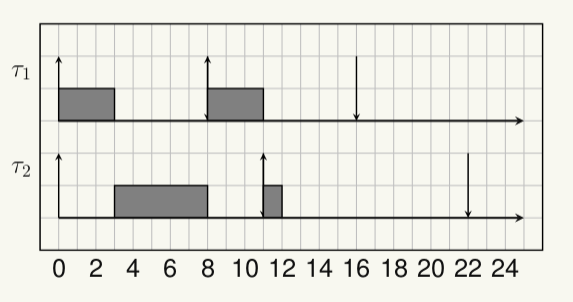
\includegraphics[width = 0.75\textwidth]{images/image14}
    \caption{}
    \label{fig:image14}
\end{figure}

Using EDF the task set is schedulable as seen in figure \ref{fig:image15}
\begin{figure}[!h]
    \centering
    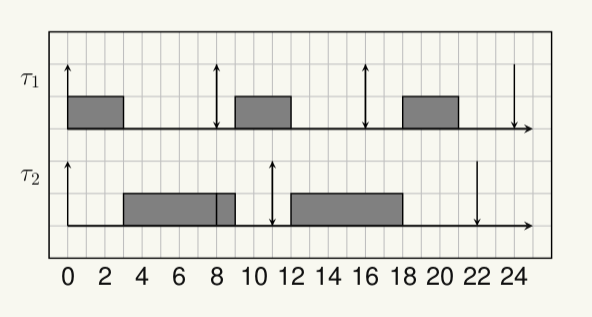
\includegraphics[width = 0.75\textwidth]{images/image15}
    \caption{}
    \label{fig:image15}
\end{figure}

EDF from a theoretically point of view solves all our problems in terms of schedulability, but most real-time operating system utilizes fixed priority assignments.\\
This is because priorities are useful for scheduling analysis and because the priority allows the developer to quantify the relative importance of a task.

    % Real time scheduling
    % Cyclic Executive Scheduling
    % Fixed Priority Scheduling
    %   RM - DM
    % Dynamic Priority Scheduling
    %   EDF
    
    % How to schedule aperiodic/sporadic tasks in parallel to periodic tasks using fixed priorities
    \chapter{Aperiodic Servers}
The scheduling algorithms treated in the previous chapter deals with homogeneous sets of tasks, where all computational activities are periodic. Many real-time control applications, however, require both aperiodic and periodic processes, which may also differ for their criticality. Tipically, periodic tasks are time-driven and execute critical control activities with hard timing contraints aimed at guaranteeing regular activation rates. Aperiodic tasks are usually event-driven and may have hard, soft, or non real-time requirements depending on the specific applications.

When dealing with hybrid task sets, the main objective of the kernel is to guarantee the schedulability of all critical tasks in worst-case conditions and provide good average response times for soft and non-real-time activities. Off-line guarantee of event-driven aperiodic tasks with critical timing contraints can be done only by making proper assumptions on the environment; that is, by assuming a maximum arrival rate for each critical event. This implies that aperiodic tasks associated with critical events are characterized by a minimum interarrival time between consecutive instances, which vounds the aperiodic load. Aperiodic tasks characterized by a minimum interarrival time are called sporadic. They are guaranteed under peak-load situations by assuming their maximum arrival rate.

\section{Background Execution}
The simplest method to handle a set of soft aperiodic activities in the presence of periodic tasks is to schedule them in background; that is, when there are not periodic instances ready to execute. The major problem with this technique is that, for high periodic loads, the response time of aperiodic requests can be too long for certain applications. For this reason, background scheduling can be adopted only when the aperiodic activities do not have stringest timing constraints and the periodic load is not high.

The major advantage of background scheduling is its simplicity. In general, only two queues are needed to implement the scheduling mechanism: one (with a higher priority) dedicated to periodic tasks and the other (with a lower priority) reserved for aperiodic requests. The two queueing strategies are independent and can be realized by different algorithms. Tasks are taken from the aperiodic queue only when the periodic queue is empty. The activation of a new periodic instance causes any aperiodic tasks to be immediately preempted.

    \begin{figure}[!h]
        \centering
        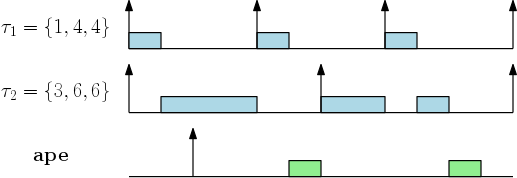
\includegraphics[width = 0.75\textwidth]{images/image02.png}
    \end{figure}

\section{Immediate Execution}
Contrary to the Background Execution, aperiodic tasks are served with the highest priority as soon as they come. This however, might cause deadline misses among the periodic tasks.

\begin{figure}[!h]
    \centering
    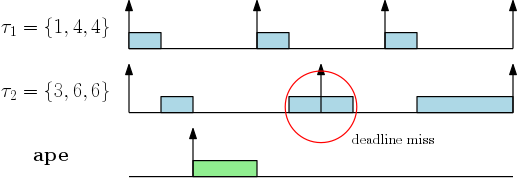
\includegraphics[width = 0.75\textwidth]{images/image03.png}
\end{figure}

Aperiodic Servers are the solution to the problem. Normally we associate two parameters with a server:
\begin{itemize}
    \item $C_s$: capacity
    \item $T_s$: server period
\end{itemize}
Roughly speaking, the idea is that the served tasks receive no more that $C_s$ time units every $T_s$. How this is done depends on the specific server technology.


The server is scehduled as any periodic tasks. Priorities are manipulated in favour of the server. Tasks inside the server can be queued with an arbitrary discipline.
\section{Polling Servers (PS)}
The average response time of aperiodic tasks can be improved with respect to background scheduling through the use of a \side{server}, that is, a periodic task whose purpose is to service aperiodic requests as soon as possible. Like any periodic task, a server is characterized by a \side{server period} $T_s$ and a computation time $C_s$, called \side{server capacity}, or \side{server budget}. In general, the server is scheduled with the same algorithm used for the periodic tasks, and once active, it serves the aperiodic requests within the limit of its budget. The ordering of aperiodic requests does not depend on the scheduling algorithm used for periodic tasks, and it can be done by arrival time, computation time, deadline or any other parameter.


\begin{figure}[!h]
    \centering
    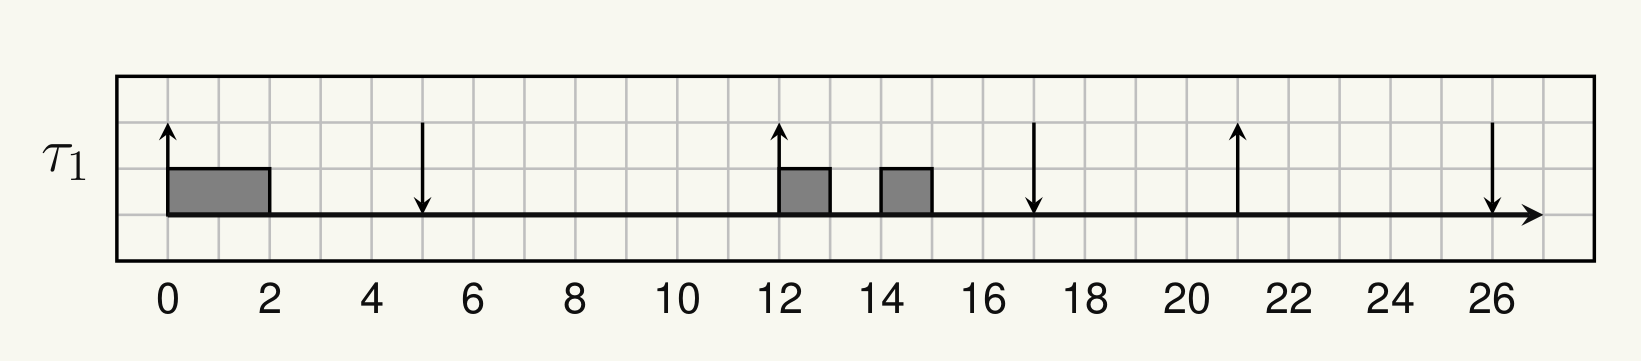
\includegraphics[width = 0.75\textwidth]{images/image04.png}
\end{figure}


The \side{Polling Server (PS)} is an algorithm based on such an approach. At regular intervals equal to the period $T_s$, PS become active and serves the pending aperiodic requests withing the limit of its capacity $C_s$. If no aperiodic requests are pending, PS suspends itself until the beginning of its next period, and the budget originally allocated for aperiodic service is discharged and given periodi tasks.\\
Note that if an aperiodic request arrives just after the server has suspended, it must wait until beginning of the next period, when the server capacity is replenished at its full value.

\section{Deferrable Servers (DS)}
The \side{Deferrable Server (DS)} algorithm is a service technique introduced by Lehoczky, Sha, and Strosnider to improve the average response time of aperiodic requests with respect to polling service. As the Polling Server, the DS algorithm creates a periodic task (usually having a high priority) for servicing aperiodic requests. However, unlike polling, DS preserves its capacity if no requests are pending upon the invocation of the server. The capacity is maintained until the end of the period, so that aperiodic requests can be services at the same server's priority at anytime, as long as the capacity has not been exhausted. At the beginning of any server period the capacity is replenished at its full value.


\begin{figure}[!h]
    \centering
    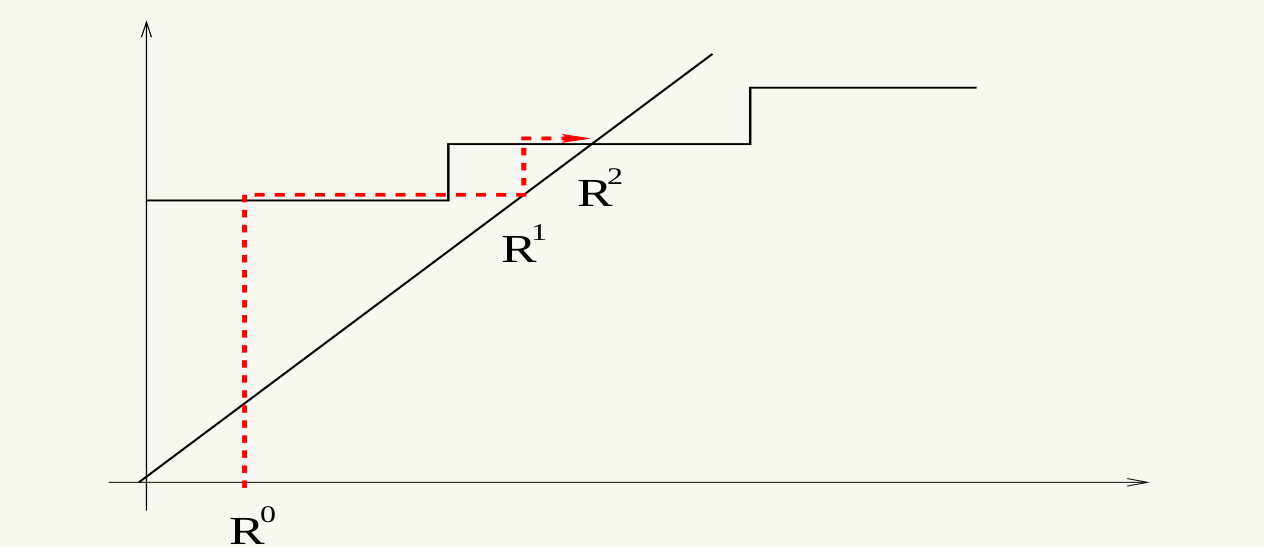
\includegraphics[width = 0.75\textwidth]{images/image05.png}
\end{figure}


DS provides much better aperiodic responsiveness than polling, since it preserves the capacity until is needed. Shorter response times can be achieved by creating a Deferrable Server having the highest priority among the periodic tasks.

\section{Sporadic Servers (SS)}

The \side{Sporadic Server (SS)} algorithm is another technique which allow the enhancement of the average response time of aperiodic  tasks without degrading the utilization bound of the periodic task set.

The SS algorithm creates a high-priority task for servicing aperiodic requests and, like DS, preserves the server capacity at its high-priority level until an aperiodic request occurs. However, SS differs from DS in the way it replenishes its capacity. Whereas DS periodically replenish their capacity to full value at the beginning of each server period, SS replenishes its capacity only after it has been consumed by aperiodic task execution.

In order to simplify the description of the replenishment method used by SS, the following terms are defined:
\begin{itemize}
    \item{\makebox[1.5cm]{$P_{exe}$\hfill} It denotes the priority level of the task that is currently executing}
    \item{\makebox[1.5cm]{$P_{s}$\hfill} It denotes the priority level associated with SS}
    \item{\makebox[1.5cm]{\textbf{Active}\hfill}SS is said to be active when $P_{exe}\ge P_s$}
    \item{\makebox[1.5cm]{\textbf{Idle}\hfill}SS is said to be idle when $P_{exe} < P_s$}
    \item{\makebox[1.5cm]{\textbf{RT}\hfill} It denotes the replenishment time at which the SS capacity will be replenished}
    \item{\makebox[1.5cm]{\textbf{RA}\hfill}It denotes the replenishment amount that will be added to the capacity at time RT}
\end{itemize}

Using this terminology, the capacity $C_s$ consumed by aperiodic requests is replenished according to the following rules:
\begin{itemize}
    \item The replenishment time RT is set as soon as SS becomes active and $C_s > 0$. Let $t_a$ be such a time. The value of RT is set equal to $T_a$ plus the server period
     \[RT = t_a + T_s\]
    \item The replenishment amount RA to be done at time RT is computed when SS becomes idle or $C_s$ has been exhausted. Let $t_I$ be such ta time. The value of RA is set equal to the capacity consumed withing the interval $[t_a, t_I]$ 
\end{itemize}

\section{Constant Bandwidth Servers (CBS)}
In this section we present a novel service mechanism, called \side{Constant Bandwidth Server (CBS)}, which efficiently implements a bandwidth reservation strategy. The Constant Bandwidth Server guarantees that, if $U_s$ is the fraction of processor time assigned to a server (i.e. its bandwidth), its contribution to the total utilization factor is no greater thatn $U_s$, even in the presence of overloads. 

The basic idea behind the CBS mechanism can be explained as follows: when a new job enters the system, it is assigned a suitable scheduling deadline (to keep its demand within the reserved bandwidth) and it is inserted in the EDF ready queue. If the job tries to execute more than expected, its deadline is postponed (i.e. its priority is decreased) to reduce the interference on the other tasks. Note that by postponing the deadline, the task remains eligible for execution. In this way, the CBS behaves as a work conserving algorithm, exploiting the available slack in an efficient (deadline-based) way, thus prividing better responsiveness with respect to non-work conserving algorithms and to other reservation approaches that schedule the extra portions of jobs in background.

If a subset of tasks is handled by a single server, all the tasks in that subset will share the same bandwidth, so there is no isolation among them. Novertheless, all the other tasks in the system are protected agains overruns occurring in the subset.

In order not to miss any hard deadline, the deadline assignment rules adopted by the server must be carefully designed.

\definition{Constant Bandwidth Server}{
    A CBS is characterized by three main quantities:
    \begin{itemize}
        \item an ordered pair $(Q_s, T_s)$ assigned by the user.\\
        Where $Q_s$ is the maximum budget and $T_s$ is the period of the server. The ratio
        \[U_s = \cfrac{Q_s}{T_s}\]
        is denotes as the server bandwidth.
        \item The current budget $q_s$ (initialized to 0) managed by the server.
        \item The scheduling deadline $d_s$ (initialized to 0) managed by the server.
    \end{itemize}
    Each served job $J_k$ is assigned a dynamic deadline equal to the current server deadline.\\
    Whenever a served job executes, the server budget $q_s$ is decreased by the same amount.
}

The CBS acts considering the following procedures:
\begin{enumerate}
    \item When the server budget is exhausted (i.e. $q_s = 0$), the server budget is recharged at the maximum value $Q_s$ and a new server deadline is generated as $d_s = d_s + T_s$. Note that there are no finite intervals of time in which the budget is equal to zero.
    \item When a job $J_k$ arrives and the server is active the request is enqueued in a queue of pending jobs according to a given (arbitrary) discipline.
    \item When a job $J_k$ arrives and the server is idle, if $q_s \ge (d_s - r_k) U_s$ the server generates a new deadline $d_s = r_k + T_s$ and $q_s$ is recharged at the maximum value $Q_s$, otherwise the job is served with the last server deadline $d_s$ using the current budget.
    \item When a job finishes, the next pending job, if any, is served using the current budget and deadline. If there are no pending jobs, the server becomes idle.
\end{enumerate}

Hence, the server behaviour can be described by the algorithm:
\begin{algorithm}
    \begin{algorithmic}
        \STATE At arrival of job $J_k$ at time $r_k\,\rightarrow$ Assign $d_s$ 
        \IF{$\exists$ pending aperiodic request}
        \STATE enqueue $J_k$
        \ELSE
        \IF{($q_s \ge (d_s - r_k)\,U_s$)}  % not enough budget left
        \STATE $q_s \leftarrow Q_s$       % replanish the budget
        \STATE $d_s \leftarrow r_k + T_s$ % generate new deadline
        \ELSE
        \STATE Continue to use the budget $q_s$ with deadline $d_s$
        \ENDIF
        \ENDIF
    \end{algorithmic}
\end{algorithm}

\begin{figure}[!h]
    \centering
    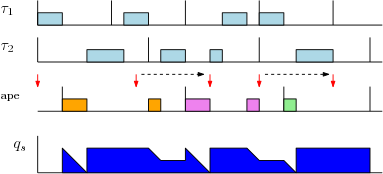
\includegraphics[width= 0.75\textwidth]{images/image10.png}
    \caption{Example of two periodic task and CBS with $(Q_s, T_s) = (2,6)$. The priority ordering is $\tau_1 > CBS > \tau_2$}
\end{figure}


\subsection{CBS Properties}
The proposed CBS service mechanism presents some interesting properties that make it suitable for supporting applications with highly variable computation times. The most important one, the \side{temporal isolation property}, is formally expressed as follows:

\theorem{}{The CPU utilization of a CBS with parameters $(Q_s, T_s)$ is 
\[U_s = \cfrac{Q_s}{T_s}\]
 independently from the computation times and the arrival pattern of the served jobs.}

 \lemma{}{Given a set of $n$ periodic hard tasks with processor utilization $U_p$ and a set of $m$ CBSs with processor utilization 
 \[U_s = \sum_{i=1}^m U_{si}\]
 the whole set is schedulable by EDF if and only if
 \[U_p + U_s \le 1\]
 }

 The temporal isolation property allows us to use a bandwidth reservation strategy to allocate a fraction of the CPU time to soft tasks whose computation time cannot be easily bounded. The most imporant consequence of this result is that soft tasks can be scheduled together with hard tasks without affecting the a priori guarantee, even in the case in which the execution time of the soft tasks are not known or the soft requests exceed the expected load.\\
 Another general technique used in real-time systems for limiting the effects of overruns in tasks with variable computation times is the \side{resource reservation paradigm}. According to this method, each task is assigned a fraction of the processor bandwidth, just enough to satisfy its timing containts. The kernel, however, must prevent each task from consuming more that the requested amount to protect the other tasks in the systems (\side{temporal protection}). In this way, a task receiving a fraction $U_i$ of the total processor bandwidth behaves as it were executing alone on a slower processor with a speed equal to $U_i$ times the full speed. The advantage of this method is that each task can be guaranteed in isolation, independently of the behavior of the other tasks.

 A simple and effective mechanism for implementing resource reservation in a real-time system is to reserve each task $\tau_i$ a specified amount of CPU time $Q_i$ in every reservation period $T_s$.



    % Background execution
    % Immediate execution
    % Polling server
    % Deferrable server
    % Sporadic Server
    % Constant Bandwidth servers
    % CBS + EDF

    \chapter{Resource Access Protocols}
\section{Introduction}
A \side{resource} is any software structure that can be used by a process to advance its executino. Tipically,  a resource can be a data structure, a set of variables, a main mamory area, a file, or a set of registers of a peripheral device. A resource dedicated to a particular process is said to be \textit{private}, whereas a resource that can be used by more tasks is called a \textit{shared resource}. A shared resource protexted against concurrent accesses is called an \textit{exclusive resource}.

To ensure consistency of the data structures in exclusive resources, any concurrent operating system should use appropriate resource access protocols to guarantee a mutual exclusion among competing tasks. A piece of code executed under mutual exclusion contraints is called a \side{critical section}.

Any task that needs to enter a critical section must wait until no other task is holding the resource. A task waiting for exclusive resource is said to be \textit{blocked} on that resource, othertwise it proceeds by entering the critical section and holds the resource. When a task leaves a critical section, the resource associated with the critical section becomes \textit{free}, and it can be allocated to another waiting task, if any.

In this chapter, we describe the main problems that may arise in a uniprocessor system when concurrent tasks use shared resources in exclusive mode, and we present some resource access protocols designed to avoid such problems and bound the maximum blocking time of each task. We then show how such blocking times can be used in the schedulability analysis to extend the guaranteee tests derived for periodic task sets.

\subsection{Atomicity}
So far we have assumed that all tasks that run and compete for a processor are independent, which means that they do not interact with one another. But there are several occasions in which this assumption cannot be made (e.g. when two tasks need to share information, exchange variables,\dots).
The other is when you have to compete for shared resources.

In this section we will introduce this problem and in particular we will introduce the notion of atomicity.
\definition{Atomic Instruction}{An atomic instruction is an instruction whose execution cannot be interleaved with the execution of other instructions}
In this sense atomic operations are always sequentialized since they cannot be interrupted. Under these conditions they are safe operations.\\
On the other hand, non atomic operations can be interrupted, and as such they are not \textit{safe} operations.

Usually, it is preferrable to have, whenever possible, non atomic operations, because they allow you to exploit in full the possibility of scheduling the processor to activities having higher priority via preemption.

\example{Non atomic operations}{
    Conside a simple operation like 
    \[x = x+1\]
    The variable is stored in a memory address that we call $x$. Hence, whenever the variable is incremented using this operation, we would have to:
    \begin{itemize}
        \item load the variable $x$ into a register $R0$
        \begin{center}
        \texttt{LD  R0, x}
        \end{center}
        \item increment the register
        \begin{center}
            \texttt{INC  R0}
        \end{center}
        \item store back the value contained in the register into $x$
        \begin{center}
        \texttt{ST  x, R0}
        \end{center}
    \end{itemize}
}
If the same operation is executed inside an interrupt handler an inconsistency may arise.

\example{Interrupt on non-atomic operations}{
Let us consider that the increment operation is both applied in the normal code and in an interrupt handler code (routine executed in response to an interrupt).\\
In both cases, the operation is translated into the assembly language using three instructions (load, increment and store).

The program starts executing as follows:
\begin{enumerate}
    \item The normal code starts executing: the value of $x$ is loaded from memory to the register
    \item At some point during this operation something triggers the execution of the interrupt
    \item The interrupt handler creates a copy of all the registers
    \item The interrupt handler load (once again) $x$ from memory, increments the register and stores the result in memory (the value of $x$ in memory has changed to $x+1$)
    \item Upon the interrupt handler has completed, the saved registers are restored. Hence, the old value of the register (i.e. $x$) is loaded back, its value is incremented to $x+1$ and stored into memory at the address of $x$ 
\end{enumerate}
The problem is that even though the code should have performed two increments (i.e. the final value should have been $x+2$), it yields the incorrect result (i.e. $x+1$).

From a logical point of view two increment operations should have taken place, but in effect one of them not successfully completed because while i was incrementing the variable, I was allowed to be interrupted and I was left with a state that was not up to date.
}

The nasty problem about this phenomenon is that it does not always happen in this way, because sometimes the function successfully completes before the interrupt is fired.\\
The example provided is the description of a condition called \side{critical race}, because you can have multiple execution of your code that interleave the operation in slightly different ways and you obtain different results.

This is a nasty problem in computer science because it might not materialize for years.

This is so because you cannot make assumption about the speed of the hardware and on the exact moment when certain events take place (we do not know the order of execution of the hardware instructions).

The case studies proposed are a perfect example of a not atomic operation that should be atomic.

The same behaviour occurs not only in the case of interrupts but also on interleaving tasks: so you could have two tasks running in parallel, both of which are sharing the variable $x$.

We can give a few definitions that are important for the follow up of our discussion:
\definition{Shared Object}{An object where the conflict may happen.}
\definition{Critical section}{A critical section is a sequence of operations that cannot be interleaved with other operations on the same resource}
\definition{Mutual exclusion}{Two critical sections cannot be active at the same time (they must be sequentialized). Either one or the other needs to stand by while the other executes}

There are three ways to obstain mutual exclusion:
\begin{enumerate}
    \item Implementing the critical section as an atomic operation.\\
    This that interrupt are disabled before the execution of the critical section and then are restored upon termination of the operation. The problem with this is that it is really tough because disabling the interrupts the I/O system of the machine is no longer allowed to work properly. (pressing an emergency button will have no effect and the execution of the code will continue),\\
    Moreover if the critical section is long, no interrupt can arrive during the critical section. In the case of a timer interrupt that arrives every 1ms, if a critical section lasts more than 1ms, a timer interrupt could be lost!
    \item Disabling the preemption (system-wide).\\
    This strategy will have some problems, because all the tasks will suffer from this suspention of the preemption even though they do not use shared resources.
    \item Selectively disabling the preemption (using semaphores and mutual exclusion).\\
    This strategy will disable preemption only for the task that operates on the shared resource.
\end{enumerate}
Hence, we should try to disable preemption rather than disabling interrupts.

Still the big issue with selectively disabling preemption the priority mechanism is no longer enforced: during the critical section might force the process to execute low priority tasks because preemption is disabled. This phenomenon is known as \side{Priority Inversion}.

If Priority inversion is not correctly managed it may lead to a complete violation of all timing contraints.
\subsection{Interacting Tasks}
Until now, we have considered only independent tasks, which are characterized by the fact that a job never blocks or suspends and a task only blocks on job termination.\\
In the real world, jobs might block for various reasons:
\begin{itemize}
    \item Tasks exchange data throught shared memory (mutual exclusion)
    \item A task might need to synchronize with other tasks while waiting for some data
    \item A job might need a hardware resource which is currently not available.
\end{itemize}

\example{Control Application}{
    Let us consider a control application composed by three periodic tasks:
    \begin{itemize}
        \item $\tau_1$ reads the data from the sensors and applies a filter. The results are stored in memory.
        \item $\tau_2$ reads the filtered data and computes some control law (updating the state and the outputs); both the state and the outputs are stored in memory
        \item $\tau_3$ reads the outputs and writes on an actuator
    \end{itemize}
    All of the three tasks access data in shared memory. This means that there are conflicts on accessing this data concurrently with the risk that the data structures become inconsistent.
    }

\subsection{Priority Inversion Phenomenon}

The rest of this chapter presents the following resource access protocols:
\begin{itemize}
    \item Non-Preemptive Protocol (NPP)
    \item Highest Locking Priority (HLP)
    \item Priority Inheritance Protocol (PIP)
    \item Priority Ceiling Protocol (PCP)
\end{itemize}

\section{Non Preemptive Protocol (NPP)} 
A simple solution that avoids the unbounded priority inversion problem is to disallow preemption during the execution of any critical section. This method, also referred to as \side{Non-Preemptive Protocol (NPP)}, can be implemented by raising the priority of a task to the highest priority level whenever it enters a shared resource. In particular, as soon as a task $\tau_i$ enters a resource $R_k$, its synamic priority is raised to the level:
\[p_i(R_k) = \max_h \{p_h\}\]
The dynamic priority is then reset to the nominal value $p_i$ when the task exits the critical section.

\begin{figure}[!h]
    \centering
    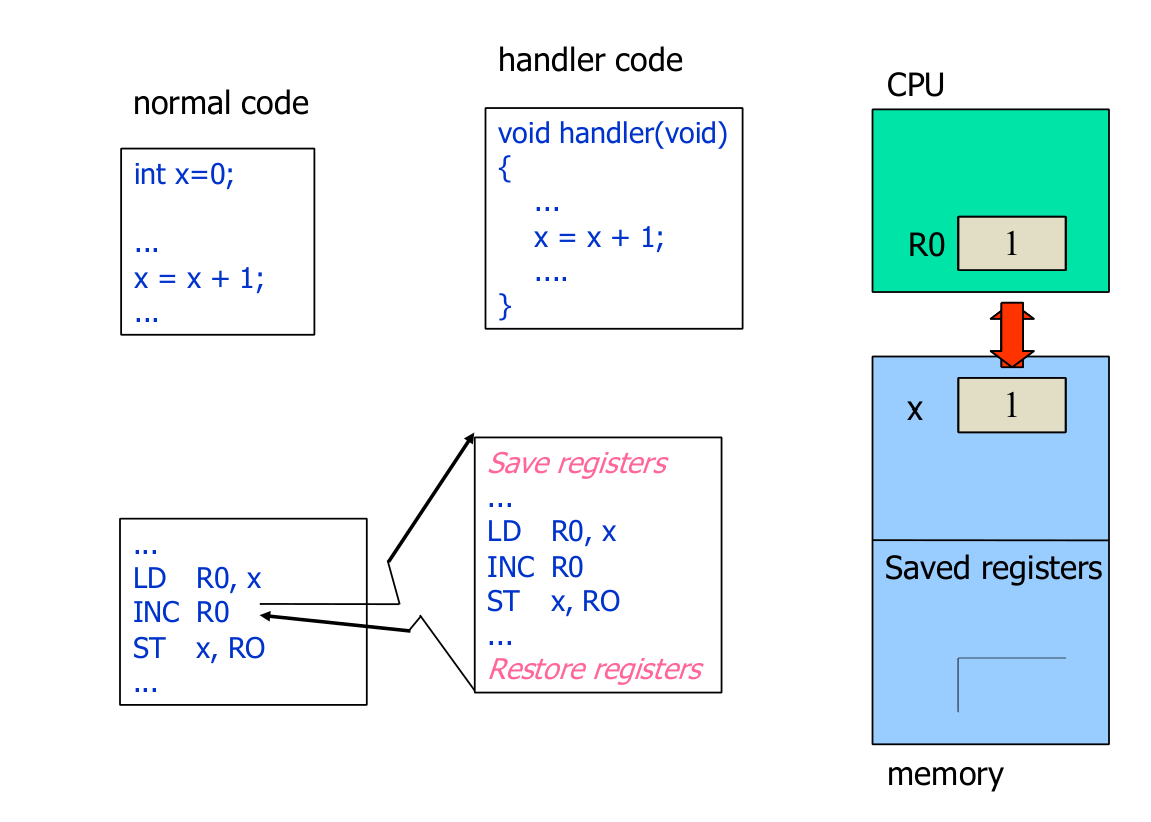
\includegraphics[width =0.75\textwidth]{images/image06.png}
\end{figure}


This method solves the priority inversion phenomenon, however, is only appriopriate when tasks use short critical sections because it creates unnecessary blocking. This actually might cause deadline misses of tasks that do not use the shared resource.

\begin{figure}[!h]
    \centering
    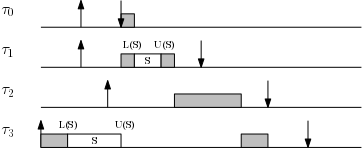
\includegraphics[width =0.75\textwidth]{images/image07.png}
\end{figure}
In the example, $\tau_0$ misses its deadline (suffers a blocking time equal to 3) even though it does not use any resource!!\\
The solution is to raise $\tau_3$ priority to the maximum between tasks accessing the shared resource (i.e. $\tau_1$) priority.



\section{Highest Locking Priority (HLP)}
The \side{Highest Locking Priority (HLP)} protocol improves NPP by raising the priority of a task that enters a resource $R_k$ to the highest priority among the tasks sharing that resource. In particular as soon as a task $\tau_i$ enters a resource $R_k$, its dynamic priority is raised to the level
\begin{equation}
\label{eq:equation2}
p_i(R_k) = \max_h\{p_i | \tau_h \text{ uses } R_k\}
\end{equation}

The dynamic priority is then reset to the nominal value $p_i$ when the task exits the critical section. The online computation of the priority level in equation \ref{eq:equation2} can be simplified by assigning each resource $R_k$ a \side{priority ceiling} $C(R_k)$ (computed offline) equal to the maximum priority of the tasks sharing $R_k$; that is:
\[C(R_k) = \max_h\{p_i | \tau_h \text{ uses } R_k\}\]
Then, as soon as a task $\tau_i$ enters a resource $R_k$, its dynamic priority is raised to the ceiling of the resource. For this reason, this protocol is also referred to as \side{Immediate Priority Ceiling}.

\begin{figure}[!h]
    \centering
    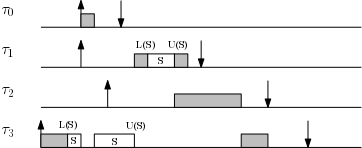
\includegraphics[width =0.75\textwidth]{images/image08.png}
\end{figure}

\section{Priority Inheritance Protocol (PIP)}
The \side{Priority Inheritance Protocol (PIP)} proposed by Sha, Rajkumar and Lehoczky, avoids unbounded priority inversion by modifying the priority of those tasks that cause blocking. In particular, when a task $\tau_i$ blocks one or more higher-priority tasks, it temporarily assumes (\textit{inherits}) the highest priority of the blocked tasks. This prevents medium-priority tasks from preempting $\tau_i$ and prolonging the blocking duration experienced by the higher-priority tasks.

The Priority Inheritance Protocol can be defined as follow:
\begin{itemize}
    \item Tasks are scheduled based on their active priorities. Tasks with the same priority are executed in a First Come First Served discipline.
    \item When task $\tau_i$ tries to enter a critical section and resource $R_k$ is already held by a lower-priority task $\tau_j$, then $\tau_i$ is blocked. $\tau_i$ is said to be blocked by the task $\tau_j$ that holds the resource. Otherwise, $\tau_i$ enters the critical section.
    \item When a task $\tau_i$ is blocked, it transmits its active priority to the task $\tau_j$ that holds the semaphore/mutex. Hence, $\tau_j$ resumes adn executes the rest of its critical section with a priority $p_j = p_i$. Task $\tau_j$ is said to inherit the priority of $\tau_i$. In general, a task inherits the highest priority of the tasks it blocks. That is, at every instant,
    \begin{equation}
        \label{eq:equation3}
        p_j(R_k) = \max \{P_j, \max_h \{P_h | \tau_h \text{ is blocked on }R_k\}\}
    \end{equation}
    \item When $\tau_j$ exits a critical section, it unlocks the mutex/semaphore, and the highest-priority task blocked, if any, is awakened. Moreover, the avtive priority of $\tau_j$ is updated as follows: if no other tasks are blocked by $\tau_j$, $p_j$ is set to its nominal priority $P_j$; otherise it is set to the highest priority of the tasks blocked by $\tau_j$, according to equation \ref{eq:equation3}.
    \item Priority inheritance is transitive; that is, if a task $\tau_3$ blocks a task $\tau_2$, and $\tau_2$ blocks a task $\tau_1$, then $\tau_3$ inherits the priority of $\tau_1$ via $\tau_2$
\end{itemize}

A high priority task can experience two kinds of blocking: \side{Direct blocking} and \side{Push-through blocking}.


\definition{Direct blocking}{It occurs when a higher-priority task tries to acquire a resource already held by a lower-priority task. Direct blocking is necessary to ensure the consistency of the shared resources}
\definition{Push-through blocking}{It occurs when a medium-priority task is blocked by a low-priority task that has inherited a higher priority from a task it directly blocks. Push-through blocking is necessary to avoid unbounder priority inversion}


\begin{figure}[!h]
    \centering
    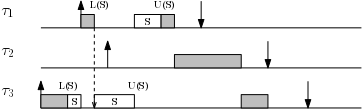
\includegraphics[width =0.75\textwidth]{images/image09.png}
\end{figure}

Although the Priority Inheritance Protocol bounds the priority inversion phenomenon, the blocking duration for a task can still be substantial because a chain of blocking can be formed. Another problem is that protocol does not prevent deadlocks (however, the latter problem can be solved by imposing a total ordering on the mutex accesses).

\section{Priority Ceiling Protocol (PCP)} % follow lecture
The \side{Priority Ceiling Protocol (PCP)} was introduced by Sha, Rajkumar, and Lehoczky to bound the priority inversion phenomenon and prevent the formation of deadlocks and chained blocking.

The basic idead of this method is to extend the Priority Inheritance Protocol with a rule granting a lock request on a free mutex. To avoid multiple blocking, this rule does not allow a task to enter a critical seciton if there are locked mutexes that could block it. This means that once a task enters its first critical section, it can never be blocked by lower-priority tasks until its completion.

In order to realize this idea, each mutex is assigned a priority ceiling equal to the highest priority of the tasks that can lock it. Then, a task $\tau_i$ is allowed to enter a critical section only if its priority is higher than all priority ceiling of the mutexes currently locked by tasks other than $\tau_i$.
\subsection{Original Priority Ceiling Protocol (OPCP)}

The \side{Original Priority Ceiling Protocol} can be defined as follows:

\subsection{Immediate Priority Ceiling Protocol (IPCP)}
    % Notion of atomicity
    % Critical sections
    % Interacting Tasks
    % Dealing with Priority inversion
    % NPP
    % HLP
    % Priority Inheritance Protocol
    \stopcontents[parts]
    
    \part{Operating System Structure}
    \startcontents[parts]
    \printcontents[parts]{}{-1}{\setcounter{tocdepth}{5}}
    \chapter{The Kernel}

Recall the following elementary defintions:
\definition{Real-Time Operating Sytems (RTOS)}{Operating System providing support to Real-Time applications}
\definition{Rea-Time application}{The correctness depends not only on the output values, but also on the time when such values are produced}
\definition{Operating System}
{
    An Operating System is:
    \begin{itemize}
        \item Set of computer programs
        \item Interface between applications and hardware
        \item a way to control the execution of application programs
        \item a way to manage the hardware and software resources
    \end{itemize}
}
In particular we can interpret an operating system as a:
\begin{itemize}
    \item a Service Provider: an API plus some services behind. This API needs to be suitable for real-time application.
    \item a Resource Manager: implements schedulers, policies to share resource, aperiodic servers, \dots
\end{itemize}
The services provided by the Operating System are executed in \side{Kernel Space}: whenever you execute a program on the operating systems the processor switches in a particular mode called \side{supervisor mode} (in this mode the processor can do anything allowed by the machine including interrupts, manage memory, \dots).
In this kernel space the operating system is able to:
\begin{itemize}
    \item Process Synchronization, Inter-Process Communication
    \item Schedule processes/threads
    \item Input and Output
    \item Allocate Virtual Memory
\end{itemize} 
All of these things are exported and accessible by means of an API.

\section{Introduction}
The core of the machine is called the \side{Kernel}
\definition{Kernel}{core part of the OS, allowing multiple tasks to run on the same CPU}
The core feature of the kernel is that it allows a task set $\mathcal{T}$ composed by $N$ tasks to run in parallel in a $M$ CPUs ($M < N$). From the application/program point of view there is no difference between having a task executed in an intermediate way or having tasks executed in a dedicated processor: so what the operating system does is to ensure a proper temporal multiplexing between the tasks.

The task scheduling service relies on two core components:
\begin{itemize}
    \item \side{Scheduler}: decides which task to execute
    \item \side{Dispatcher}: component that implements the context switch between the tasks. Often this component relies on some hardware extension that facilitates this type of service.
\end{itemize}

The kernel also provides a mechanism for allowing tasks to communicate and synchronize between each other. On this regard there are two possible paradigms: 
\begin{itemize}
    \item Shared memory (threads).\\
    Shared Memory utilizes mutexes, semaphores and condition variables, which the kernel provides. From a real time point of view this service has to come along some real-time resource sharing protocols.
    \item Message passing (processes).\\
    Contrary to Shared memory, Message passing is based on different interaction models such as pipeline, client-server, \dots\\
    The kernel must once again provide some IPC mechanism: pipes, message queues, mailboxes, remote procedure calls (RPC), \dots\\
    On top of this some real-time protocols can still be used
\end{itemize}

In practice, an adequate scheduling of system resources removes the need for over-enginnering the system, and is necessary for providing a predictable QoS. For this reason, an adequate scheduling of system resources considers two important aspects: the algorithm and the implementation.\\
For instance, we have seen efficient algorithm for scheduling tasks and resources, however all applications are treated by a \side{Timer}. 
This introduces a set of questions and problems to consider in the implementation of the scheduling algorithm:
\begin{itemize}
    \item Is the timer reliable?
    \item Is the scheuduler able to select a high-priority task as soon as it is ready?
    \item And the dispatcher?
\end{itemize}
\example{Periodic Task}{
    When considering a periodic task, it expects to be executed at time $r = r_0 + jT$, but sometimes it is delayed to $r = r_0 + jT + \delta$, where the quantity $\delta$ becomes an offset or a drift term that makes the timing not reliable.\\
    This delay may cause deadline misses.
}

\section{Kernel Latency}
\definition{Kernel Latency}{Delay $\delta$ with which a kernel implement its decisions}
When a primitive is called, the primitive takes some time to execute and during this time there is not possibility preempt the kernel. Therefore, in practice, the operating system is temporarily sospending the scheduling mechanism. This is situation really similar to the resource access protocols, in fact, we can think of the kernel as a shared resource that is not preemptable and therefore the kernel latency can be modelled as a blocking time.\\
Hence the schedulability analysis tools introduced are modified as follows:
\begin{itemize}
    \item \textbf{Processor Utilization factor test}
     \[\forall i \in [1,n] \qquad\sum_{k=1}^{i-1} \cfrac{C_k}{T_k} + \cfrac{C_i + \delta}{T_i} \le U_{lub}\]
    \item \textbf{Response Time Analysis}
    \[R_i = C_i + \delta + \sum_{h=1}^{i-1}\ceil{\cfrac{R_i}{T_h}}C_h\]
    \item \textbf{Processor Demand analysis}
    \[\exists 0\le t\le D_i\qquad W_i(0,t) = C_i \sum_{h=1}^{i-1}\ceil{\cfrac{t}{T_h}}C_h \le t-\delta\] 
\end{itemize}

The scheduler is called whenever an internal (e.g. IPC, signal, \dots) or external (e.g. interrupt) events is triggered.\\
When one of these events take place, there exists some time between the triggering of the event and the dispatch which can be decomposed in four components:
\begin{itemize}
    \item Event generation 
    \item Event delivery (interrupts may be disabled)
    \item Scheduler activation (non preemptable section)
    \item Scheduling time
\end{itemize}
There are quite a few elements that may generate the delay.

All these elements of uncertainty need to be understood, the reason and how the system manages introduces this delay and most importantly how to manage this delay in a real-time kernel.\\
Remember that we are interested in the worst case possibility, so all the components that compose the kernel latency should be designed so that in the worst-case the maximum is minimized.

\section{System Architecture}
%%%%%%%%%%%%%%%%%%%%%%%%%%%%%%%%%%%%%%%%%%%%%%%%%%%%%%%%%%%%%%%%%%%%%%%%%%%%%%%%%%%%
The system architecture is composed by a system bus that is interconnecting the following components:
\begin{itemize}
    \item One or more CPUs
    \item Memory (RAM)
    \item I/O Devices
    \begin{itemize}
        \item Secondary memory (disks, \dots)
        \item Network cards
        \item Graphic cards
        \item Keyboard, mouse, \dots
    \end{itemize}
\end{itemize}

\subsection{The CPU}
The model of the CPU is composed of the following registers
\begin{itemize}
    \item General-purpose registers that can be accessed by all the programs. These registers can be either data registers or address registers
    \item Program Counter (PC) aka Intruction pointer
    \item Stack Pointer (SP) register
    \item Flags register (aka Program Status Word)
    \item Some special registers, which control how the CPU works, must be "protected" 
\end{itemize}

Regual user programs should not be allowed to influence the CPU mode of operation, perform I/O operations and reconfigure virtual memory. For this reason there is a need for privileged mode of execution
\begin{itemize}
\item Regual registers vs special registers
\item Regual intructions vs privileged instructions
\end{itemize}
User programs: low privilge level (\side{User Level})

The OS kernel runs in supervisor mode.

\example{Intel x86}{
    Real CPUs are more complex.
    They have few General Purpose registers: EAX, EBX, ECX, EDX (accumulator registers containing an 8 bit part and a 16 bit part), EBP, ESI, EDI
    \begin{itemize}
        \item EAX: Main accumulator
        \item EBX: sometimes used as base for arrays
        \item ECX: sometimes used as counter
        \item EBP: stack base pointer (for subroutines calls)
        \item ESI: source index
        \item EDI: destination index
    \end{itemize} 
    They also have segmented memory architecture: segment registers CS (code segment), DS (data segment), SS (stack segment), GS, FS.

    Finally they have various mode of operation: RM, PM, VM86, x86-64,\dots, mainly due to backward compatibility.
}

The Kernel is part of the OS which manages the hardware.

Runs with the CPU in Supervisor Mode (high privilege level):
\begin{itemize}
    \item Privilege level known as Kernel Level (KL), execution in Kernel Space
    \item Regual programs run in User Space
\end{itemize}
Mechanismns for increasing the privilege level (from US to KS) in a controlled way
\begin{itemize}
    \item Interrupts (+ traps/hw exeptions).
    \item Instructions causing a hardware exception
\end{itemize}
Switch the CPU from User Level to Supervisor mode by entering the kernel. This can be used to implement system calls.
A partical Context Switch is performed: flags and PC are pushed to the stack, if the processor is executing at User Level, switch to Kernel Level, and eventually switch to a kernel stack finally execution jumps to a handler in the kernel (save the user registers for restoring them later).
Once finished return to low privilege level (execution returns to User Space) through a "return from interrupt" Assembly instruction (\texttt{IRET} on x86): Pop flags and PC from stack and eventually switch back to user stack.
Return path  from system calls and hardware interrupts to handlers.

To understand interrupts, copnsider simplified CPU execution first
\missingfigure{slide 24}
The CPU interatively:
\begin{itemize}
    \item Fetch an instruction (address given by PC)
    \item Increase the PC
    \item Execute the intruction (might update the PC on jump\dots)
\end{itemize}

A More realistic execution model
\missingfigure{slide 25}
Interrupt cannot fire during the execurtion of an intruction.
Hardware exception: cause by the execution of an intruction:
\begin{itemize}
    \item \texttt{trap},\texttt{syscall},\texttt{sc},\dots
    \item I/O instructions at low privilege level, Page faults, \dots
\end{itemize}

The interrupt tabole holds the addresses of the handlers:
\begin{itemize}
    \item Interrupt $n$ fires: after eventually switching to KS and pushing flags and PC on the stack
    \item Read the address contained in the $n^{th}$ entry of the interrupt table, and jump to it!
\end{itemize}

Interrupt tables are implemented in hardware or in software:
\begin{itemize}
    \item x86, interrupt description table composed by interrupt gates. The CPU automatically jumpts to the $n^{th}$ interrupt gate
    \item Other CPUs jump to a fixed address: a software demultiplexer reads the interrupt table
\end{itemize}
 

\textbf{Software Interrupt - System Call}
\begin{enumerate}
    \item Task $\tau_1$, executes and invokes a system call
    \item Execution passes from US to KS (change stack, push PC and flags, increase privilege level)
    \item The invoked syscall executes. Maybe, it is blocking
    \item $\tau_1$ blocks and the system returns to US, and $\tau_2$ is scheduled
\end{enumerate}

\textbf{Hardware Interrupt}
\begin{enumerate}
    \item Task $\tau_2$ is executing, a hardware interrupt fires
    \item Execution passes from US to KS (change stack, push PC and flags, increase privilege level)
    \item the proper Interrupt Service Routine executes
    \item The ISR can unblock $\tau_1$. When execution returns to US, $\tau_1$ is scheduled
\end{enumerate}

The executino flow enters the kernel for two reasons
\begin{itemize}
    \item Reacting to events coming from up (syscalls)
    \item Reacting to an event coming from below (an hardware interrupt from a device)
\end{itemize}
The kernel executes in the context of the interrupted task.\\
A system call can block the invoking task, or can unblock a different task\\
An ISR can unblock a task\\
If a task is blocked/unblocked, when returning to user space a context switch can happen.

The scheduler is invoked when return from KS to US

\example{I/O operation}{Consider a generic Input or Output to an external device such as a PCI card.\\
This operation is performed by the kernel and user programs must uyse a syscall

The operation is performed in 3 phases:
\begin{enumerate}
    \item Setup: prepare the device for the I/O operation
    \item Wait: wait for the end of  the operation
    \item Cleanup: complete the operation
\end{enumerate}
This can be done using polling, PIO, DMA, \dots
}

\subsection{Polling}
    User programs invoke the kernel; execution in kernel space until the operation is terminated.\\
    The kernel cyclically reads (polls) an interafce status register to check if the operation is terminated\\
    Busy-waiting in kernel space!
    \begin{itemize}
        \item No user task can execute while waiting for the I/O operation \dots
        \item The operation must be very short
        \item I/O operation == blocking time
    \end{itemize} 

    \begin{enumerate}
        \item The user program raises a software input
        \item Setup phase - in kernel: in case of input operation, nothing is done; in case of output operation, write a value to a card register
        \item Wait - in kernel: cycle until a bit of the card status register becomes 1
        \item Cleanup - in kernel: in case of input, read a value from a card register; in case of output, nothing is done. Eventually return to phase 1
        \item IRET
    \end{enumerate}
    \subsection{Programmed I/O}
    User programs invoke tyhe kernel; execution returns to user space while waiting for the device: the task that invoked the syscall blocks\\
    Anb interrupt will notify the kernel when the "wait" phase is terminated:
    \begin{itemize}
        \item The interrupt handler will take care of performing the I/O operation
        \item Many frequent short interruption of unrelated user-space tasks
    \end{itemize}

    \begin{enumerate}
        \item The user program raises a software input
        \item Setup phase - in kernel: instruct the device to raise an input when it is ready for I/O
        \item Wait - return to user space: block the invoking task, and schedule a new one (IRET)
        \item Cleanup - in kernel: the interrupt fires $\rightarrow$ enter kernel, and perform the I/O operation
        \item Return to phase 2, or unblock the task if the operation is terminated (IRET)
    \end{enumerate}
\subsection{DMA}
User programs invoke the kernel; execution returns to user space while waiting for the device. The task that invoked the syscall blocks!

I/O operations are not performed by the kernel on interrupt, Performed by a dedicated HW device,\\
An interrupt is raised when the whole I/O operation is terminated

\begin{enumerate}
    \item The user program raises a software input
    \item Setup phase - in kernel: instruct the DMA (or the Bus Mastering Device) to perform the I/O
    \item Wait - return to user space: block the invoking task, and schedule a new one (IRET)
    \item Cleanup - in kernel: the interrupt fires $\rightarrow$ the operation is terminated. Stop device and DMA
    \item Unblock the task and invoke the scheduler (IRET)
\end{enumerate}
    \chapter{Timer and Clock Latency}
\definition{Latency}{Measure of the diffence between the theoretical and actual schedule.}
\example{}{A task $\tau$ expects to be scheduled at time $t$, but is actually scheduled at time $t'$.
The resulting latency $L$ takes the form:
\[L = t' - t\]
}

The latency $L$ can be modelled as a blocking time and as such affects the guarantee test.
Similar to what done for shared resources. \\
Blocking time due to latency, not to priority inversion.

Upper bound for $L$? if not known, no schedulability tests!!
The latency must be bounded:
\[\exists L^{max}: L < L^{max}\]
If $L^{max}$ is too high, only few task sets result ot be schedulable.\\
Large blocking time experienced by all tasks!\\
The worst-case latency $L^{max}$ cannot be too high.

A task $\tau_i$ is a stream of jobs $J_{i,j}$ arriving at time $r_{i,j}$.\\
Job $J_{i,j}$ is schedulable at time $t' > r_{i,j}$\\
$t' - r_{i,j}$ is given by:
\begin{enumerate}
    \item $J_{i,j}$'s arrival is signalled at time $r_{i,j} + L^1$
    \item Such event is served at time $r_{i,j} + L^1 + L^2$
    \item $J_{i,j}$ is actually scheduled at $r_{i,j} + L^1 + L^2 + L^3$
\end{enumerate}
where:
\begin{itemize}
    \item $L^1$ is due to the delayed interrupt generation.\\
    Hardware interrupts; generated by devices.\\
    Sometimes, an interrupt should be generated at time $t$ but it is actually generated at time $t' = t + L^{int}$ where $L^{int}$ iis the Interrupt Generation Latency.
    Such latency is due to hardware issues and it is generally small compared to $L^{np}$.
    The only exception is if the device is a timer device, the interrupt generation latency can be quite high
    Timer resolution latency $L^{timer}$
    \item $L^2$ is the non-preemptable section latency ($L^{np}$).\\
    Delay between time when an event is generated and when the kernel handles it.\\
    Due to non-preemptable sections in the kernel, which delay the response to hardware interrupts.\\
    It is composed by various parts: interrupt disabling, bottom halves dealying,\dots\\
    It depends on how the kernel hadles the various events,\dots
    \item $L^3$ is the scheduler latency. Which is the interference from higher priority tasks and its already accounted by the guarantee tests. Hence it will not be considered
\end{itemize}

The Timer Resolution Latency is the interrupt generation latency for a hardware timer device.\\
$L^{timer}$ can often be much larger that the non-preemptable section latency $L^{np}$.\\
Where does it come from? Kernel timers are generally implemented by using a hardware device that produces periodic interrupts.\\
Can we do anything about it?\\
A Periodic timer interrupt is called a tick\\
Example: periodic task (\texttt{setitimer()}, Posix timers, \texttt{clock\_nanosleep()},\dots) $\tau_i$ with period $T_i$\\
Job end $\rightarrow$ $\tau_i$ sleeps for the next activation.\\
Activations are triggered by the periodic interrupt:
\begin{itemize}
    \item Periodic tick interrupt, with period $T^{tick}$
    \item Every $T^{tick}$, the kernel checks if the task must be woken up
    \item If $T_i$ is not multiple of $T^{tick}$, $\tau_i$ experiences a timer resolution latency
\end{itemize}

Traditional operating systems: timer device programmed to generate a periodic interrupt.
\example{}{In a PC, the Programmable Interval Timer (PIT) is programmed in periodic mode}

At every tick the execution enter kernel space.\\
The kernel executes and can:
\begin{itemize}
    \item Wake up tasks
    \item Adjust tasks priorities
    \item Run the scheduler, when returning to user space (possible preemption)
\end{itemize}

Timer interrupt period: trade-off between responsiveness (low latency) and throughput (low overhead).
\begin{itemize}
    \item Large $T^{tick}$: large timer resolution latency
    \item Small $T^{tick}$: high number of interrupts.\\
More switches between US and KS, tasks are interrupted more often and a resulting large overhead
\end{itemize}

For non real-time systems, it is possible to find a reasonable tradeoff but it still depends on the workload.
\example{Linux Kernel}
{
    \begin{itemize}
        \item Linux 2.4: 10 ms (100Hz)
        \item Linux 2.6: 100 Hz, 250 Hz or 1000Hz
        \item Other systems: $T^{tick} = \sfrac{1}{1024}$
    \end{itemize}
}
The timer resoultion latency is experienced by all tasks that want to sleep for a specified time $T$.\\
$\tau_i$ must wake up at time $r_{i,j} = j T_i$, but is woken up at time $t' = \ceil{\cfrac{r_{i,j}}{T^{tick}}}T^{tick}$.

The Timer Resolution Latency is bounded:
\begin{itemize}
    \item $t = r_{i,j}$
    \item $t' = \ceil{\cfrac{r_{i,j}}{T^{tick}}}T^{tick}$
\end{itemize}
\begin{align*}
    L^{timer} &= t' - r_{i,j}\\
&= \ceil{\cfrac{r_{i,j}}{T^{tick}}}T^{tick}- r_{i,j}\\
&= \left(\ceil{\cfrac{r_{i,j}}{T^{tick}}} - \cfrac{r_{i,j}}{T^{tick}}\right) T^{tick} \le T^{tick}
\end{align*}

Reducing $T^{tick}$ below 1ms is generally not acceptable, so periodic tasks can expect a blocking time due to $L^{timer}$ up to 1ms.
How loarge is the effect on the schedulability tests?\\
Additional problems:
\begin{itemize}
    \item Tasks' periods are rounded to multiples of $T^{tick}$
    \item Limit on the minimum task period: $\forall i, T_{i}\ge T^{tick}$
    \item A lot of useless timer interrupts might be generated
\end{itemize}

Remember?
\definition{Timer}{generate an event at a specified time $t$}
\definition{Clock}{keep track of the current system time}

A timer can be used to wake up a periodic task $\tau$, a clock can be used to read the system time (\texttt{gettimeofday()})

\definition{Timer Resolution}{minimum interval at which a periodic timer can fire. If periodic ticks are used, the timer resolution is $T^{tick}$}
\definition{Clock Resolution}{minimum difference between two different timer returned by the clock.}
What's the expected clock resolution?
\begin{itemize}
    \item Traditional OSs use a "tick counter". \\
    Very fast clock: return the number of ticks (jiffies in Linux) from the system boot\\
    Clock resolution : $T^{tick}$
    \item Modern PCs have higher resolution time sources\dots\\
    On x86, TSC (TimeStamp Counter)\\
    High-resolution clock: use the TSC to compute the time since the last timer tick\dots
    \item In summary: high-resolution clocks are easy: every modern OS kernel provide them.
    \item Even using a "traditional" periodic timer tick, it is easy to provide high-resolution clocks: time can be easily read with a high accuracy. 
    \item On the other hand, timer resolution is limited by the system tick $T^{tick}$. It is impossible to generate events at arbitrary instants in time, without latencies
\end{itemize}


\section{Timer Devices}
Timer Devices (e.g. PIT - i8254) generally work in 2 modes: periodic and one-shot.\\
Programmed writing a value $C$ in a counter register.\\
The counter register is decremented at a fixed rate.\\
When the counter is 0, an interrupt is generated:
\begin{itemize}
    \item If the device is programmed in periodic mode, the counter register is automatically reset to the programmed value
    \item If the device is programmed in one-shot mode, the kernel has to explicitly reprogram the device (setting the counter register to a new value)
\end{itemize}

The periodic mode is easier to use! This is why most kernels use it.\\
When using one-shot mode, the timer interrupt handler must:
\begin{enumerate}
    \item Acknowledge the interrupt handlerm, as usual
    \item Check if a timer expired, and do its usual stuff\dots
    \item Compute when the next timer must fire
    \item Reprogram the timer device to generate an interrupt at the correct time
\end{enumerate}
Steps 3 and 4 are particularly critical and difficult.\\
When the kernel reprograms the timer device (step 4), it must know the current time, but the last known time is the time when the interrupt fired (before step 1):
\begin{itemize}
    \item A timer interrupt fires at time $t_1$
    \item The interrupt handler starts (enter KS) at time $t_1'$
    \item Before returning to US, the timer must be reprogrammed, at time $t_1''$
    \item Next interrupt must fire at time $t_2$; the counter register is loaded with $t_2 - t_1$
    \item Next interrupt will fire at $t_2 + (t_1'' - t_1)$
\end{itemize}
The error described previously accumulates with the risk of drift between real time and system time.\\
A free run counter (not stopped at $t_1$) is needed.\\
The counter is synchronised with the timer device and the value of the counter at time $t_1$ is known.\\
This permits to know the time $t_1''$. The new counter register value can be computed correctly.\\
On a PC, the second PIT counter, or the TSC, or the APIC timer can be used as a free run counter.

Serious real-time kernels use high-resolution timers (use hardware time in one-shot mode) which for instance is already implemented in RT-Mach, RTLinux, RTAI and others.\\
General purpose kernels are more concerned about stability and overhead.

Compatibility with "traditional" kernels:
\begin{itemize}
    \item The tick event can be emulated through high-resolution timers
    \item Timer device programmed to generate interrupts both: when needed to serve a timer and at tick boundaries but the "tick" concept is now useless (e.g. Tickless or NO\_HZ system which are good for saving power)  
\end{itemize}
    \chapter{The Non Preemptable Section Latency}
    \stopcontents[parts]

    
    \part{Additional information and proofs}
    \startcontents[parts]
    \printcontents[parts]{}{-1}{\setcounter{tocdepth}{5}}
    \appendix
    \chapter{$U_{lub}$ for RM for $N$ tasks}
Given a task set $\mathcal{T}$ of $N$ tasks scheduled using the RM priority assignment, the conditions that allow to compute the least upper bound of the processor utilization factor are:
\[
\begin{dcases}
    T_1 < T_n < 2T_1\\
    C_1 = T_2 - T_1\\
    C_2 = T_3 - T_2\\
    \dots\\
    C_{n-1} = T_n - T_{n-1}\\
    C_n = T_1 - \sum_{i=1}^{n-1}C_i = 2T_1 - T_n
\end{dcases}    
\]
Thus the processor utilization factor becomes
\[T = \cfrac{T_2 - T_1}{T_1} + \cfrac{T_3- T_2}{T_2} + \dots + \cfrac{T_n- T_{n-1}}{T_{n-1}} + \cfrac{2T_1 - T_n}{T_n}\]
Defining
\[R_i = \cfrac{T_{i+1}}{T_i}\]
and noting that 
\[\prod_{i=1}^{n-1} R_i= \cfrac{T_n}{T_1}\]
the utilization factor may be written as 
\[U = \sum_{i=1}^{n-1}R_i + \cfrac{2}{\prod_{i=1}^{n-1} R_i} - n\]

To minimize $U$ over $R_i$, $i = 1,\dots, n-1$, we have
\[\pd{U}{R_k} = 1 - \cfrac{2}{R_i\,\prod_{i=1}^{n-1} R_i}\]
Thus defining $P = \prod_{i=1}^{n-1} R_i$, $U$ is minimum when:
\[
    \begin{dcases}
        R_1 P = 2\\
        R_2 P = 2\\
        \dots\\
        R_{n-1}P = 2
    \end{dcases}
\]
that is, when all $R_i$ have the same value
\[R_1 = R_2 = \dots = R_{n-1} = 2^{\sfrac{1}{n}}\]
Substituting this value in $U$ we obtain
\begin{align*}
    U_{lub} &= (n-1)2^{\sfrac{1}{n}} + \cfrac{2}{2^{(1 - \sfrac{1}{n})}} - n\\
    &= n 2^{\sfrac{1}{n}} - 2^{\sfrac{1}{n}} + 2^{\sfrac{1}{n}} -n\\
    &= n(2^{\sfrac{1}{n}} - 1)
\end{align*}
    \chapter{$U_{lub}$ for RM + Polling Server}
We first consider the problem of guaranteeing a set of hard periodic tasks in the presence of soft aperiodic tasks handled by a Polling Server. Then we show how to derive a schedulability test for hard aperiodic requests.

The schedulability of periodic tasks can be guaranteed by evaluating the interference introduced by the Polling Server on periodic execution. In the worst case, such an interference is the same as the one introduced by an equivalent periodic task having a periodi equal to $T_s$ and a computation time equal to $C_s$. In fact, independently of the number of aperiodic tasks handled by the server, a maximum time equal to $C_s$ is dedicated to aperiodic requests at each server period. As a consequence, the processor utilization factor of the Polling Server is
\[U_s = \cfrac{C_s}{T_s}\]
and hence the schedulability of a periodic set with $n$ tasks and utilization $U_p$ can be guaranteed if
\[U_p + U_s \le U_{lub}(n+1)\]
If periodic tasks (including the server) are scheduled by RM, the schedulability test becomes
\[\sum_{i=1}^{n} \left(\cfrac{C_i}{T_i}\right) + \cfrac{C_s}{T_s} \ le (2^{\sfrac{1}{(n+1)}}- 1)(n+1)\]
Note that more Polling Servers can be created and execute concurrently on different aperiodic task sets.\\
In general, in the presence of $m$ servers, a set of $n$ periodic tasks is schedulable by RM if
\[U_p + \sum_{j=1}^m U_sj \le U_{lub}(n+m)\]
A more precise schedulability test can be derived by assuming that PS is the highest-priooority task in the system. To simplify the computation, the worst-case relations among the tasks are first determined, and then the lower bound is computed against the worst-case model.

Consider a set of $n$ periodic tasks ($\tau_1,\dots, \tau_n$) ordered by increasing periods, and a PS server with highest priority. The worst-case scenario for a set of periodic tasks that fully utilize the processor is characterized by the following parameters:
\[
\begin{dcases}
    C_s = T_1 - T_s\\
    C_1 = T_2 - T_1\\
    C_2 = T_3 - T_2\\
    \dots\\
    C_{n-1} = T_n - T_{n-1}\\
    C_n = T_s - C_s - \sum_{i=1}^{n-1}C_i = 2T_s - T_n
\end{dcases}    
\]

The resulting utilization is then
\begin{align*}
    U &= \cfrac{C_s}{T_s} + \cfrac{C_1}{T_1} + \dots + \cfrac{C_n}{T_n}\\
    &= U_s + \cfrac{T_2 - T_1}{T_1} + \dots + \cfrac{T_n - T_{n-1}}{T_{n-1}} + \cfrac{2T_s - T_n}{T_n}\\
    &= U_s + \cfrac{T_2}{T_1} + \dots + \cfrac{T_n}{T_{n-1}} + \left(\cfrac{2T_s}{T_1}\right) \cfrac{T_1}{T_n} - n 
\end{align*}

Defining:
\[
    \begin{dcases}
        R_s = \cfrac{T_1}{T_s}\\
        R_i = \cfrac{T_{i+1}}{T_i}\\
        K = \cfrac{2T_s}{T_1} = \cfrac{2}{R_s}
    \end{dcases}
\]
and noting that 
\[R_1R_2\dots R_{n-1} = \prod_{j=1}^{n-1}R_j = \cfrac{T_n}{T_1}\]
The utilization factor may be written as
\[U = U_s + \sum_{i=1}^{n-1}R_i + \cfrac{K}{\prod_{j=1}^{n-1}R_j} - n\]
we minimize $U$ over $R_i$, $i = 1,\dots,n-1$. Hence,
\begin{align*}
    \pd{U}{R_i} &= \cancelto{0}{\pd{U_s}{R_i}} - \cancelto{0}{\pd{n}{R_i}} + \cancelto{0}{\pd{\sum_{j\ne i}^{n-1} R_j}{R_i}} + \pd{R_i}{R_i} + \pd{K\,\left(\prod_{j=1}^{n-1}R_j\right)^{-1}}{R_i}\\
    &= 1 + K\,\left(\prod_{j=i}^{n-1}R_j\right)^{-1}\,\pd{R_i^{-1}}{R_i}\\
    &= 1 - K\,\left(\prod_{j=i}^{n-1}R_j\right)^{-1}\,R_i^{-2}\\
    &= 1 - \cfrac{K}{R_i^2\,\left(\prod_{j\ne i}^{n-1}R_j\right)}\\
    &= 1 - \cfrac{K}{R_i \, \left(\prod_{j=1}^{n-1}R_j\right)}
\end{align*}

Thus, defining $P= \prod_{j=1}^{n-1}R_j$, U is minimum when:

\[
\begin{dcases}
    R_1P = K\\
    R_2P = K\\
    \dots\\
    R_{n-1}P = K
\end{dcases}
\]
that is, when all $R_i$ have the same value:
\[R_1 = R_2 = \dots = R_{n-1} = K^{\sfrac{1}{n}}\]
Substituting this value in $U$ we obstain:
\begin{align*}
    U_{lub} &= U_s + \sum_{i=1}^{n-1}R_i + \cfrac{K}{\prod_{j=1}^{n-1}R_j} - n\\
    &= U_s +\sum_{i=1}^{n-1}\left(K^{\sfrac{1}{n}}\right) + \cfrac{K}{\prod_{j=1}^{n-1}\left(K^{\sfrac{1}{n}}\right)} - n\\
    &= U_s + (n-1)K^{\sfrac{1}{n}} + \cfrac{K}{K^{\sfrac{n-1}{n}}}-n\\
    &= U_s + (n-1)K^{\sfrac{1}{n}} + K\,K^{-\sfrac{n-1}{n}}-n\\
    &= U_s + (n-1)K^{\sfrac{1}{n}} + K{1-\sfrac{n-1}{n}}-n\\
    &= U_s + (n-1)K^{\sfrac{1}{n}} + K{\sfrac{n-n+1}{n}}-n\\
    &= U_s + (n-1)K^{\sfrac{1}{n}} + K{\sfrac{1}{n}}-n\\
    &= U_s + nK^{\sfrac{1}{n}} - K^{\sfrac{1}{n}} + K{\sfrac{1}{n}} - n\\
    &= U_s + n(K^{\sfrac{1}{n}} - 1)
\end{align*}

Now, noting that 
\[U_s = \cfrac{C_s}{T_s} = \cfrac{T_1-T_s}{T_s} = R_s - 1\]
we have
\[R_s = U_s + 1\]
Thus, $K$ can be rewritten as
\[K = \cfrac{2}{R_s} = \cfrac{2}{U_s + 1}\]
and finally
\[U_{lub} = U_s + n \left[\left(\cfrac{2}{U_s + 1}\right)^{\sfrac{1}{n}}-1\right]\]

Thus, given a set of $n$ periodic tasks and a polling server withg utilization factors $U_p$ and $U_s$, respectively, the schedulability of the periodic task set is guaranteed under RM if
\[U_p + U_s \le U_s + n\left(K^{\sfrac{1}{n}} - 1\right)\]
that is, if
\[U_p \le n \left[\left(\cfrac{2}{U_s + 1}\right)^{\sfrac{1}{n}}-1\right]\]
    \chapter{$U_{lub}$ for RM + Deferrable Server}
To simplify the computation of the bound for $n$ periodic tasks, we first determine the worst-case relations among the tasks, and then we derive the lower bound against the worst-case model.

Consider a set $n$ periodic tasks ($\tau_1,\dots, \tau_n$), ordered by increasing periods, and a Deferrable Serve with a higher priority. The worst-case condition for the priodic tasks, is such that $T_1 < T_n < 2T_1$. In the presence of a DS, however, the derivation of the worst-case is more complex and requires the analysis of three different cases. For the sake of clarity, here we analyze one case only, the most general, in which DS may execute three times within the period of the highest-priority periodic task. This happens when DS defers its service at the end of its period and lso executes at the beginning of the next period. In this situation, the full processor utilization is achieved by the following tasks' parameters:

\[
\begin{dcases}
    C_s = T_1 - (T_s + C_s) = \cfrac{T_1 - T_s}{2}\\
    C_1 = T_2 - T_1\\
    C_2 = T_3 - T_2\\
    \dots\\
    C_{n-1} = T_n - T_{n-1}\\
    C_n = T_s - C_s - \sum_{i=1}^{n-1}C_i = \cfrac{3T_s + T_1 - 2T_n}{2}
\end{dcases}    
\]

Hence, the resulting utilization is:
\begin{align*}
    U &= \cfrac{C_s}{T_s} + \cfrac{C_1}{T_1} + \dots + \cfrac{C_n}{T_n}\\
    &= U_s + \cfrac{T_2 - T_1}{T_1} + \dots + \cfrac{T_n - T_{n-1}}{T_{n-1}} + \cfrac{3T_s + T_1 - 2T_n}{2T_n}\\
    &= U_s + \cfrac{T_2}{T_1} + \dots + \cfrac{T_n}{T_{n-1}} + \left(\cfrac{3T_s}{2T_1} + \cfrac{1}{2}\right) \cfrac{T_1}{T_n} - n 
\end{align*}

defining:
\[
    \begin{dcases}
        R_s = \cfrac{T_1}{T_s}\\
        R_i = \cfrac{T_{i+1}}{T_i}\\
        K = \cfrac{1}{2}\left(3\cfrac{T_s}{T_1} + 1\right)
    \end{dcases}
\]
and noting that 
\[R_1R_2\dots R_{n-1} = \prod_{j=1}^{n-1}R_j = \cfrac{T_n}{T_1}\]
The utilization factor may be written as
\[U = U_s + \sum_{i=1}^{n-1}R_i + \cfrac{K}{\prod_{j=1}^{n-1}R_j} - n\]
we minimize $U$ over $R_i$, $i = 1,\dots,n-1$. Hence,
\begin{align*}
    \pd{U}{R_i} &= \cancelto{0}{\pd{U_s}{R_i}} - \cancelto{0}{\pd{n}{R_i}} + \cancelto{0}{\pd{\sum_{j\ne i}^{n-1} R_j}{R_i}} + \pd{R_i}{R_i} + \pd{K\,\left(\prod_{j=1}^{n-1}R_j\right)^{-1}}{R_i}\\
    &= 1 + K\,\left(\prod_{j=i}^{n-1}R_j\right)^{-1}\,\pd{R_i^{-1}}{R_i}\\
    &= 1 - K\,\left(\prod_{j=i}^{n-1}R_j\right)^{-1}\,R_i^{-2}\\
    &= 1 - \cfrac{K}{R_i^2\,\left(\prod_{j\ne i}^{n-1}R_j\right)}\\
    &= 1 - \cfrac{K}{R_i \, \left(\prod_{j=1}^{n-1}R_j\right)}
\end{align*}

Thus, defining $P= \prod_{j=1}^{n-1}R_j$, U is minimum when:

\[
\begin{dcases}
    R_1P = K\\
    R_2P = K\\
    \dots\\
    R_{n-1}P = K
\end{dcases}
\]
that is, when all $R_i$ have the same value:
\[R_1 = R_2 = \dots = R_{n-1} = K^{\sfrac{1}{n}}\]
Substituting this value in $U$ we obstain:
\begin{align*}
    U_{lub} &= U_s + \sum_{i=1}^{n-1}R_i + \cfrac{K}{\prod_{j=1}^{n-1}R_j} - n\\
    &= U_s +\sum_{i=1}^{n-1}\left(K^{\sfrac{1}{n}}\right) + \cfrac{K}{\prod_{j=1}^{n-1}\left(K^{\sfrac{1}{n}}\right)} - n\\
    &= U_s + (n-1)K^{\sfrac{1}{n}} + \cfrac{K}{K^{\sfrac{n-1}{n}}}-n\\
    &= U_s + (n-1)K^{\sfrac{1}{n}} + K\,K^{-\sfrac{n-1}{n}}-n\\
    &= U_s + (n-1)K^{\sfrac{1}{n}} + K{1-\sfrac{n-1}{n}}-n\\
    &= U_s + (n-1)K^{\sfrac{1}{n}} + K{\sfrac{n-n+1}{n}}-n\\
    &= U_s + (n-1)K^{\sfrac{1}{n}} + K{\sfrac{1}{n}}-n\\
    &= U_s + nK^{\sfrac{1}{n}} - K^{\sfrac{1}{n}} + K{\sfrac{1}{n}} - n\\
    &= U_s + n(K^{\sfrac{1}{n}} - 1)
\end{align*}

Now, noting that 
%

\[U_s = \cfrac{C_s}{T_s} = \cfrac{T_1-T_s}{2T_s} = \cfrac{R_s - 1}{2}\]
we have
\[R_s = 2U_s + 1\]
Thus, $K$ can be rewritten as
\[K = \left(\cfrac{3}{2R_s} + \cfrac{1}{2}\right) = \cfrac{U_s + 2}{2U_s + 1}\]
and finally
\[U_{lub} = U_s + n \left[\left( \cfrac{U_s + 2}{2U_s + 1}\right)^{\sfrac{1}{n}}-1\right]\]

Thus, given a set of $n$ periodic tasks and a polling server withg utilization factors $U_p$ and $U_s$, respectively, the schedulability of the periodic task set is guaranteed under RM if
\[U_p + U_s \le U_s + n\left(K^{\sfrac{1}{n}} - 1\right)\]
that is, if
\[U_p \le n \left[\left( \cfrac{U_s + 2}{2U_s + 1}\right)^{\sfrac{1}{n}}-1\right]\]
    \chapter{POSIX}
\section{Implementing Periodic Tasks}
The pseudocode of a Periodic Task is:
\begin{lstlisting}[language=C]
    void *PeriodicTask(void *arg)
    {
        <initialization>;
        <start periodic timer, period = T>;
        while (condition)
        {
            <job body>;
            <wait next activation>;
        }
    }
\end{lstlisting}

The job body is outside of out control as well as the initialization since it is application dependent. Hence we will analyze the various way we can implement the \texttt{<start periodic timer>} and \texttt{<wait next activation>} section/function using timers and clocks.

\subsection{Using UNIX clock}

The idea is to use unix clocks to implement the \texttt{wait\_next\_activation} function using \texttt{usleep} (relative sleep).

In this naive implementation:
\begin{itemize}
    \item The program reads the current time
    \item The program computes the relative sleep
    \[\delta = \text{next activation time} - \text{current time}\]
    \item The program calls \texttt{usleep} for a value of $\delta$
\end{itemize}

\begin{lstlisting}[language=C]
    void wait_next_activation(void)
    {
        gettimeofday(&tv, NULL);
        d = nt - (tv.tv_sec * 1000000 + tv.tv_usec);
        nt += period;
        usleep(d);
    }
\end{lstlisting}

The problem with this implementation is that preemption can happen in \texttt{wait\_next\_activation} between \texttt{gettimeofday} and \texttt{usleep} resulting in an incorrect sleeping time of the task.

The solution is to call a function that implements a periodic behaviour.

\subsection{Using UNIX itimer}
Unix systems provide a system call for setting up a periodic timer.

\begin{lstlisting}[language=C]
    #include <sys/time.h>
    int setitimer (int which, const struct itimerval *value, struct itimerval *ovalue);
\end{lstlisting}
The first parameter of the system call is the type of interval timer to use. Three values are admissible:
\begin{itemize}
    \item \texttt{ITIMER\_REAL}: timer fires after a specified real time. \texttt{SIGALRM} is sent to the process.
    \item \texttt{ITEMER\_VIRTUAL}: timer fires after the process consumes a specified amount of time (process time). \texttt{SIGPROF} is sent to the process.
    \item \texttt{ITEMER\_PROF}: process time + system calls (both user and system time = profiling)
\end{itemize}

Hence \texttt{setitimer()} can be used to implement \texttt{<start periodic timer>}.

\begin{lstlisting}[language=C]
    #include <sys/time.h>  // setitimer()
    #include <signal.h>    // signal()
    #include <unistd.h>    // pause()

    #define wait_next_activation pause // pause till a signal is fired

    static void sighand(int s) {} // empty signal handler (need for signal())

    int start_periodic_timer(uint64_t offs, int period)
    {
        struct itimerval t;
        // offset
        t.it_value.tv_sec     = offs / 1000000;
        t.it_value.tv_usec    = offs % 1000000;
        // period
        t.it_interval.tv_sec  = period / 1000000;
        t.it_interval.tv_usec = period % 1000000;
        // register signal and specify signal handler
        signal(SIGALRM, sighand);

        return setitimer(ITIMER_REAL, &t, NULL);

    }
\end{lstlisting}

The problem with this implementation is that the \texttt{SIGALRM} generated is handled by an empty handler. An idea is to implement a better \texttt{wait\_next\_activation}: instead of pause, the function can wait a \texttt{SIGALRM}.


\begin{lstlisting}[language=C]
    #include <sys/time.h>  // setitimer()
    #include <signal.h>    // signal()

    static sigset_t sigset;

    static void wait_next_activation(void)
    {
        int dummy;
        sigwait(&sigset, &dummy); // wait for any signal in the set to be pending
    }

    int start_periodic_timer(uint64_t offs, int period)
    {
        struct itimerval t;
        // offset
        t.it_value.tv_sec     = offs / 1000000;
        t.it_value.tv_usec    = offs % 1000000;
        // period
        t.it_interval.tv_sec  = period / 1000000;
        t.it_interval.tv_usec = period % 1000000;
        // define set of signal that should be processed
        sigemptyset(&sigset);                  // exclude all the defined signals
        sigaddset(&sigset, SIGALRM);           // add SIGALRM to the signal set
        sigprocmask(SIG_BLOCK, &sigset, NULL); // block signals specified in sigset (required by sigwait)

        return setitimer(ITIMER_REAL, &t, NULL);
    }
\end{lstlisting}

The limitation of using UNIX timers is that only one real-time timer is available per process.

\subsection{POSIX timers}
POSIX offer multiple types of clocks (e.g. \texttt{CLOCK\_REALTIME} and \texttt{CLOCK\_MONOTONIC}). In addition, it is possible to set up multiple timers per process (each process can dynamically allocate and start timers).
A timer firing generates an asynchronous event which si configurable by the program.

\begin{lstlisting}[language=C]
    #include <time.h> // timer_create()
    int timer_create(clockid_t clockid, struct sigevent *sevp, timer_t* timerid);
\end{lstlisting}
\begin{itemize}
    \item \texttt{clockid} specifies the clock that the new timer uses to measure time.
    \item \texttt{sevp} points to a \texttt{sigevent} structure that specifies how the caller should be notified when the timer expires
    \item \texttt{timerid} id of the new timer returned by the system call.
\end{itemize}

\begin{lstlisting}[language=C]
    #include <time.h> // timer_settime()
    int timer_settime(timer_t timerid, int flags, const struct itimerspec*v, struct itimerspec *ov);
\end{lstlisting}
\begin{itemize}
    \item \texttt{timerid} timer id
    \item \texttt{flags}: (use 0 = \texttt{TIMER\_ABSTIME})
    \item \texttt{v}: interval timer specifications (timer offset \texttt{it\_value}, timer period \texttt{it\_interval})
    \item \texttt{ov}: just set this to NULL... you wont need it trust me
\end{itemize}

Since we are using POSIX we need to link agains \texttt{librt} hence when compiling link the executable using the compiler flag \texttt{-lrt}.

With this new timer the implementation of \texttt{start\_periodic\_timer} becomes
\begin{lstlisting}[language=C]
    #include <time.h>      // timer_create(), timer_settime
    #include <signal.h>    // signal()
    #include <string.h>    // memset()

    static sigset_t sigset;

    static void wait_next_activation(void)
    {
        int dummy;
        sigwait(&sigset, &dummy); // wait for any signal in the set to be pending
    }

    int start_periodic_timer(uint64_t offs, int period)
    {
        struct itimerspec t;
        struct sigevent sigev;
        timer_t timer;
        int res;
        const int signal = SIGALRM;
        // offset
        t.it_value.tv_sec     = offs / 1000000;
        t.it_value.tv_usec    = offs % 1000000;
        // period
        t.it_interval.tv_sec  = period / 1000000;
        t.it_interval.tv_usec = period % 1000000;
        // define set of signal that should be processed
        sigemptyset(&sigset);                  // exclude all the defined signals
        sigaddset(&sigset, SIGALRM);           // add SIGALRM to the signal set
        sigprocmask(SIG_BLOCK, &sigset, NULL); // block signals specified in sigset (required by sigwait)
        // specify the sigevent
        memset(&sigev, 0, sizeof(struct sigevent)); // empty sigevent structure
        sigev.sigev_notify = SIGEV_SIGNAL;
        sigev.sigev_signo = signal;
        // create timer
        res = timer_create(CLOCK_MONOTONIC, &sigev, &timer);
        // inizialize periodic timer with the specs in t
        return timer_settime(timer, TIMER_ABSTIME, &t, NULL);
    }
\end{lstlisting}

Still a process can still be preempted and the relative sleeping problem is still present in some form. The solution is to use Absolute Time from POSIX timers and clocks

\subsection{Using POSIX clock and timers with Absolute time}
Instead of reading the current time and computing $\delta$ based on it \texttt{wait\_next\_activation()} can directly wait for the absolute arrival time of the next job using a \texttt{clock\_nanosleep()} call.
\begin{lstlisting}[language=C]
    #include <time.h>
    int clock_nanosleep(clockid_t clock_id, int flags, const struct timespec *request, struct timespec *remain);
\end{lstlisting}
\begin{itemize}
    \item \texttt{clock\_id}: specifies the clock agains which the sleep interval is to be measured (\texttt{CLOCK\_REALTIME}, \texttt{CLOCK\_MONOTONIC}, \texttt{CLOCK\_PROCESS\_CPUTIME\_ID}).
    \item \texttt{flags}: if 0 then specified request is interval, if \texttt{TIMER\_ABSTIME} then specified request is an absolute time.
    \item \texttt{request} structure specifying time to wait
    \item \texttt{remain} (if not NULL) returns the remaining unslept time
\end{itemize}
\begin{lstlisting}[language=C]
    #include <time.h>
    clock_gettime(clockid_t clk_id, struct timespec* res);
\end{lstlisting}
\begin{itemize}
    \item \texttt{clock\_id}: specifies the clock agains which the sleep interval is to be measured (\texttt{CLOCK\_REALTIME}, \texttt{CLOCK\_MONOTONIC}, \texttt{CLOCK\_PROCESS\_CPUTIME\_ID}).
    \item \texttt{res} result of the clock reading
\end{itemize}

\begin{lstlisting}[language=C]
    #include <time.h>      // clock_gettime(), clock_nanosleep()

    static struct timespec r;
    static int period;

    static inline void timespec_add_us(struct timespec *t, uint64_t d){ ... } // add d to timespec t by converting to us to ns
    static void wait_next_activation(void)
    {
        clock_nanosleep(CLOCK_REALTIME, TIMER_ABSTIME, &r, NULL);
        timespec_add_us(&r, period)
    }

    int start_periodic_timer(uint64_t offs, int period)
    {
       clock_gettime(CLOCK_REALTIME, &r);
       timespec_add_us(&r, offs);
       period = t;
       return 0;
    }
\end{lstlisting}

Notice that r and period are global variable: this is a bad idea. Hence we wrap these two variables in a struct:
\begin{lstlisting}[language=C]
    struct periodic_task
    {
        struct timespec r;
        int period;
    }
\end{lstlisting}
Whenever a new periodic task is needed: inside \texttt{start\_periodic\_timer} periodic task is initialized and its values are passed to the aforementioned function calls.

\vfill
\textbetweendoublerules{Summary}
\begin{itemize}
    \item Unix allows 1 process to have $N$ timers and 1 thread can sleep until a future time point (only relative sleep)
    \item POSIX allows 1 timer for 1 thread (RT task) and avoids the relative-sleep problem
    \item POSIX guarantees \texttt{CLOCK\_REALTIME} exists, but it is not good for real time applications: may jump forward/backward and is prone to overflow: it cannot be restarted hence it will overflow on 32 bit machine in year 2038
    \item For these reasons, use \texttt{CLOCK\_MONOTONIC} whenever possible since it is not user settable, it is restarable when the system is restarted (use it in conjunction to \texttt{clock\_gettime()})
\end{itemize}

\section{Real-Time scheduling}
\subsection{Better Statistics}
First and foremost we need to improve the statistics for each task: since now we have considered the average time over 100 jobs as a statistics. However, this measurement may still yield a misleading result.

\example{$T=D=2$}{A task $\tau$ generates 101 jobs ranging from $J_1$ to $J_{101}$.\\
All but $J_2$ start at activation time and all but $J_1$ need 1 time units to complete.  $J_1$ however finishes 3 time units after activation (deadline miss).\\
The average time printed by $J_{101}$ is 2: 1 job every 2 time units. Through the fact that $J_1$ missed its deadline caused every other job to miss its deadline.
}
In other terms we need to introduce additional statistical quantities to verify which job if any miss their deadlines: namely jitter, best and worst case response times and consecutive deadline misses.

Given a job $J_{i,k}$ of a task $\tau_i$ we need to save the following quantities:
\begin{itemize}
    \item $k$: job number
    \item $s_{i,k}$: start time of the job
    \item $f_{i,k}$: finishing time of the job
    \item $t_0$: expected time of earliest task activation (initial offset of first job activation)
    \item For every task $\tau_i$ with offset $\Phi_i$, period $T_i$ and relative deadline $D_i$, compute the absolute activation time and absolute deadline:
    \[r_{i,k} = t_0 + \Phi_i + (k-1)T_i\qquad d_{i,k} = r_{i,k} + D_i\]
    Given these quantities we can define:
    \begin{itemize}
        \item A job $J_{i,k}$ does not miss its deadline if 
        \[r_{i,k}\le s_{i,k}\le f_{i,k} \le d_{i,k}\]
        \item Best and worst case response time
        \[\min_k{(f_{i,k} - r_{i,k})}\qquad \max_k{(f_{i,k} - r_{i,k})}\]
        \item Relative start time jitter
        \[\max_k \abs{(s_{i,k} - r_{i,k}) - (s_{i,k-1} - r_{i,k-1})}\]
        \item Absolute start time jitter
        \[\max_k \abs{s_{i,k} - r_{i,k}} - \min_k{(s_{i,k} - r_{i,k})}\]
        \item Relative finish time jitter
        \[\max_k \abs{(f_{i,k} - r_{i,k}) - (f_{i,k-1} - r_{i,k-1})}\]
        \item Absolute finish time jitter
        \[\max_k \abs{f_{i,k} - r_{i,k}} - \min_k{(f_{i,k} - r_{i,k})}\]
    \end{itemize}
\end{itemize}

These quantities can be measured using the \texttt{clock\_gettime()} in conjunction with \texttt{CLOCK\_MONOTONIC}, whereas $t_0$ can be computed using \texttt{timer\_settime()} with flag \texttt{TIMER\_ABSTIME}.\\
In addition to this the response time $R_{i,k}$ is equal to the execution time $c_{i,k}$ if and only if $r_{i,k}$ up to $f_{i,k}$ has no preemption/blocking, otherwise it holds that $R_{i,k} > c_{i,k}$.
To measure the execution time use \texttt{clock\_gettime()} with \texttt{CLOCK\_THREAD\_CPUTIME\_ID}.
In addition, since this measurement is affected by energy-saving mode we need to change the cpu scaling for each core in the machine:
\begin{lstlisting}[language=bash]
    cd /sys/devices/system/cpu/cpufreq
    cat policy?/scaling_{min,cur,max}_freq   # cat scaling_{min,cur,max}_freq content contained in each folder policy$character$
    for x in policy?; do
        sudo tee $x/scaling_min_freq < $x/scaling_max_freq; % for each core policy replace scaling_min_freq with scaling_max_freq
    done
    cat policy?/scaling_{min,cur,max}_freq   # cat scaling_{min,cur,max}_freq content contained in each folder policy$character$
\end{lstlisting}

\subsection{Real-Time Scheduling}
POSIX provides support for real-time scheduling: but NO multiprocessor parititoning and migration.\\
To provide this support for real time scheduling POSIX provides priority scheduling support:
\begin{itemize}
    \item Multiple priority levels
    \item A task queue per priority level
    \item Run first task fo highest-priority in non-empty queue
\end{itemize}
POSIX also provides multiple scheduling policies: a scheduling policy describes how tasks are moved between the prioririty queues. Please notice that these scheduling policies consider Fixed priority: task is always in the same priority queue.\\
Not all RT theory for uniprocessor (UP) is for MP. So we need to partition MP to have 1 processor as 1 UP.
In order to do so we add the following api calls:
\begin{lstlisting}[language=C]
    #define _GNU_SOURCE // CPU_ZERO(), CPU_SET(), sched_setaffinity()
    #include <sched.h>  // CPU_ZERO(), CPU_SET(), sched_setaffinity()

    void main(int argc, char**argv)
    {
        cpu_set_t cpumask;
        CPU_ZERO(&cpumask);         // clears cpumask, so that it contains no CPUs
        CPU_SET(0, &cpumask);       // Add CPU 0 to cpumask
        // sets the CPU affinity mask of the thread whose ID is pid (=0),
        // if pid is zero, then the calling thread is used.
        // it also has to provide the size of the cpuset pointed to by cpumask
        if (sched_setaffinity(0, sizeof(cpumask), &cpumask))
        {
            perror("sched_setaffinity failed");
            return -1;
        }
    }
\end{lstlisting}

POSIX specifically requires four scheduling policies:
\begin{itemize}
    \item \texttt{SCHED\_FIFO}: tasks with same priority level (in the same queue) are executed in a first in first out manner (this might lead to starvation of other tasks with same priority). Only higher priotiy tasks can preempt it
    \item \texttt{SCHED\_RR}: tasks with same priority level (in the same queue) are executed in a round robin fashion: a task executes for a \side{time/scheduling quantum} (fixed interval of time), than it is suspended and added to the back of the queue (tasks with the same priority are served fairly)
    \item \texttt{SCHED\_SPORADIC}: is a sporadic server that decreases the response times of aperiodic RT tasks
    \item \texttt{SCHED\_OTHER}: is the traditional Unix scheduler. It has dynamic priorities, and it is scheduled in background with respect to fixed priorities.
\end{itemize}

RR and FIFO priority values are comparable:
\begin{itemize}
    \item \texttt{sched\_get\_priority\_min(int \$policy\$)}: lowest priority value
    \item \texttt{sched\_get\_priority\_max(int \$policy\$)}: highest priority value
\end{itemize}

Hence the schduling policy can be set using the following API calls:
\begin{lstlisting}[language=C]
    #include <sched.h>  

    int sched_get_priority_min(int policy); // minimum priority value that can be used by the policy
    int sched_get_priority_max(int policy); // maximum priority value that can be used by the policy
    
    struct sched_param
    {
        ...
        int sched_priority;
        ...
    }
    /*
        @pid:    id of the thread (if 0 calling thread)
        @policy: scheduling policy
        @param:  value between min and max priority value (for SCHED_FIFO and SCHED_RR)
    */
    int sched_setscheduler(pid_t pid, int policy, const struct sched_param *param);
    
    /*
        @pid:    id of the thread (if 0 calling thread)
        @param:  value between min and max priority value 
    */
    int sched_setparam(pid_t pid, const struct sched_param *param);

\end{lstlisting}

If there is no swap to disk, no unlucky kernel latency, and MP has no unlycky bus contention, the scheduled RT tasks will have no deadline misses.\\
In general, "regular" (\texttt{SCHED\_OTHER}) tasks are scheduled in background relative to real-time tasks. A real-time task can preempt/starve other tasks.\\
Running applications with real-time priroities requires root privileges, hence after compiling perform this bash commands:
\begin{lstlisting}[language=bash]
    sudo chown root executable # change file owner to root
    sudo chmod u+s executable  # allow root to execute the executable (not the user)
\end{lstlisting}

\subsection{Memory Swapping}
The virtual memory mechanism can swap part of the process address space to disk: Memory swapping can increase execution times, resulting in temporal unpredictability, hence it is not good for real-time application.

A non-real time task can force a memory swap. To overcome this issue RT task can lock part of its address space in memory:
\begin{itemize}
    \item Locked memory cannot be swapped out of the physical memory disk
    \item This can result in a RAM exhaustion
\end{itemize}
Memory locking can be performed only by applications having root privileges.

\begin{lstlisting}[language=C]
    #include <sys/mman.h>

    // lock pages starting at @addr with size len (in bytes)
    int mlock(const void *addr, size_t len);
    // unlock pages starting at @addr with size len (in bytes)
    int munlock(const void *addr, size_t len);
    /*
        lock entire address space in memory
        MCL_CURRENT = current address space
        MCL_FUTURE  = all memory allocated in the future
        MCL_CURRENT | MCL_FUTURE = both
    */
    int mlockall(int flags);
\end{lstlisting}


\section{Concurrency}
A process implements the notion of \side{protection} in the sense that each process has its own address space and other private resources. A process can write/read in its address space but is not allowed to touch other processes' resources: two processes can share some resources for communication, but this has to be excplicitly allowed by them!

Processes usually communicate through message passing (e.g. pipes, sockets, signals,\dots).

A process is more than a set of private resources, it is an active entity.
The concept of process involves two aspects:
\begin{itemize}
    \item \side{Protection} or resource ownership
    \item \side{Execution}\\
    A process contains at least a schedulable entity, which can access the process's resources. As such it contains all the information for the scheduling (e.g. scheduling parameters).
    Furthermore this schedulable entity is also characterized by (at least) a CPU state and a stack.
\end{itemize}


Each single-threaded process has only one thread which involves:
\begin{itemize}
    \item One address space per process
    \item One stack per process
    \item One Process Control Block (PCB) per process
    \item Other private resources
    \item One single executino flow per process
\end{itemize}

This differs from a multi-threaded process in the sense that a process can have multiple threads in it:
\begin{itemize}
    \item One address space
    \item One PCB
    \item Multiple execution flows in a single process
    \item Multiple stacks (one per thread)
    \item One Thread Control Block (TCB) per thread
\end{itemize}

\subsection{Small Summary about Processes}
The Process Memory Layout involves three major components in its private address space: User memory, Stack and Heap.
In particular, the user memory is divided into three segments:
\begin{enumerate}
    \item Initialized data segment
    \item BSS (Block Started by Symbol): uninitialized global and static variables
    \item Text segment (containing the program code)
\end{enumerate}
The heap and the stack are straightforward to understand. However, the heap is usable through \texttt{malloc} and can grow using \texttt{brk()} and \texttt{sbrk()}

Each process is identified by a process ID (PID) which is unique in the system. Each time a process is created a PID is assigned to it. The value of the PID of a process can be retrieved using \texttt{getpid(void)}, whereas the PID of a process's creator (i.e. parent) can be retrieved using \texttt{getppid(void)}

\subsubsection{Fork}
A new process can be created using the api call \texttt{fork()}. The new process (called child process) contains a copy of the parent's address space. The call has one entry point and two exit points:
\begin{itemize}
    \item In the child, 0 is returned
    \item In the parent, the PID of the child is returned
\end{itemize}
In case of error fork returns a negative value is returned.

Generally speaking \texttt{fork()} is used in the following way:
\begin{lstlisting}[language=C]
    #include <sys/types.h> // pid_t
    #include <unistd.h>    // fork
    
    pid_t child_pid = fork();
    if(child_pid < 0) { return -1 }
    if(child_pid == 0)
        // child body
    else
        // parent body 
\end{lstlisting}
Alternatively:
\begin{lstlisting}[language=C]
    #include <sys/types.h> // pid_t
    #include <unistd.h>    // fork
    #include <stdlib.h>    // exit
    
    pid_t child_pid = fork();
    if(child_pid < 0) { return -1 }
    if(child_pid == 0)
    {
        // child body
        exit(0);
    }
    // parent body 
\end{lstlisting}

Since the child address space is a copy of the parent's: the child's text segment is the same as the parent's, consequently both the parent body and the child body must be in the same executable.

\subsubsection{Exec}
To avoid this one can use the \texttt{exec()} call or any of its variants.\\
Exec is a family of functions to replace the process address space (text, data and heap) (e.g. \texttt{execl()},\texttt{execlp()},\texttt{execle()},\texttt{execv()},\texttt{execvp()}).
The basic idea of exec is that it loads a new programme and jumps to it, but does not create a new process.

An example usage of exec is as follows:
\begin{lstlisting}[language=C]
    #include <sys/types.h> // pid_t
    #include <unistd.h>    // fork
    #include <stdio.h>     // perror
    
    pid_t child_pid = fork();
    if(child_pid < 0) { return -1 }
    if(child_pid == 0)
    {
        char *args[3] = {"arg1", "arg2", "arg3"};
        execve("child_body", args, NULL);
        perror("Execve"); // check if any error has occured
        return -1;
    }
    ...
\end{lstlisting}

Some non-posix compliant systems make no distinction between program and process and only provide a fork + exec combo. POSIX also provides a \texttt{system()} function which does fork + exec (+ wait)

A process terminates when:
\begin{enumerate}
    \item It invokes either the library call \texttt{exit()} or the system call \texttt{\_exit()}
    \item It returns from its main function
    \item It is killed by some external event (e.g. a signal)
\end{enumerate}

When it terminates explicity, a process can return a result to the parent.\\
Every process can register a hook ot be called on regular process termination 
\begin{lstlisting}[language=C]
    #include <stdlib.h>    // atexit
    
    int atexit(void (*function) (void));
\end{lstlisting}
However, please note that handlers are not called if exiting with \texttt{\_exit()}.

\subsubsection{Wait}
First form of synchronization between processes is waiting for a children to return to the parent.\\
A parent can wait for its child's termination using the api calls \texttt{wait()}, \texttt{waitpid()}, \texttt{wait4()}.
Formally:
\begin{lstlisting}[language=C]
    #include <sys/types.h>    // pid_t
    #include <sys/wait.h>     // wait()
    
    pid_t wait(int *status);
\end{lstlisting}
If the calling process has no children, \texttt{wait()} returns a value < 0\\
If at least there is one terminated child, \texttt{wait()} returns the child's exit value, and child's private resources are freed\\
If there are no terminated children, \texttt{wait()} blocks the calling process.

The other variants of the wait family of function allow to select the child to wait for.

Please note that after a process terminates, its private resources are not freed until its parent performs a \texttt{wait()}. Children processes that have terminated are said to be in a \side{zombie} state. Hence a good parent has to wait for its children to terminate.
When the parent of a process dies the process is reparented to \texttt{init} (a system process whose PID is 1). As a consequence, when a process dies all its zombies are eliminated.

A process can be notified about the termination of a child process through an asynchronous event (e.g. signal: \texttt{SIGCHLD})

\subsection{synchronization through Signals}
Concurrent processes interact in different ways: competition or cooperation.\\
Cooperation can be implemented through \side{signals}: Sometimes, a process has to wait until cooperating processes have completed some operation. In other terms, a process $\tau_i$ waits for an asynchronous event generated by: another process $\tau_j$ or the system.

\definition{Signal}{Asynchronous event directed to process $\tau$. Process $\tau$ can:
\begin{itemize}
    \item Wait for a signal
    \item Perform some other work in the meanwhile, and the signal will interrupt it.
\end{itemize}}

Signals are the software equivalent of interrupts. A process receiving a signal can:
\begin{itemize}
    \item Ignore it
    \item Interrupt its execution and jump to a \side{signal handler}
    \item Abort
\end{itemize}
A signal that has not caused one of the previous actions is a \side{pending signal}.

Signals are managed using a \side{signal table}. Such structure is a per process private resource that specifies how the process handles each signal. At process creation the signal table is initialized using default values.

The table entries can be modified using: \texttt{signal()} or \texttt{sigaction()}.
\begin{lstlisting}[language=C]
    #include <signal.h>
    /*
        @signum signal (e.g. SIGALRM)
        @handler either SIG_IGN, SIG_DFL or the address of a programmer-defined function
    */

    sighandler_t signal(int signum, sighandler_t handler);
    /*
        @signum signal (e.g. SIGALRM) excluding SIGKILL and SIGSTOP
        @act    the new action for signal signum
        @oldact old action for signal signum (if not null)
    */
    int sigaction(int signum, const struct sigaction *act, struct sigaction *oldact);
\end{lstlisting}

The prototype of a signal handler is very simple: it must return void and accept an integer value as input \texttt{void sighand(int n)}.
In order to set up a signal handler, we need to provide some of the parameters in a structure \texttt{sigaction} provided by the api.

\begin{lstlisting}[language=C]
struct sigaction {
    void     (*sa_handler)(int);
    void     (*sa_sigaction)(int, siginfo_t *, void *);
    sigset_t   sa_mask;
    int        sa_flags;
    void     (*sa_restorer)(void);
};
\end{lstlisting}
where:
\begin{itemize}
    \item \texttt{sa\_handler} is the signal handler (function), or \texttt{SIG\_DFL} (default action) or \texttt{SIG\_IGN} (ignore the signal)
    \item \texttt{sa\_mask} is a mask of signals to disable when the handler runs. This set can be modified using \texttt{sigemptyset()}, \texttt{sigfillset()}, \texttt{sigaddset()}, and \texttt{sigdelset()}
    \item Running handler cannot be interrupted by the handled signal again unless \texttt{SA\_NODEFER} is set in \texttt{sa\_flags}
\end{itemize}

A process can send a signal to other processes by using 
\begin{lstlisting}[language=C]
    int kill(pid_t pid, int sig)
\end{lstlisting}
Note that it must have the proper permissions: user root can send signals to every process, other users can send signals only to their own processes.
\texttt{kill} is not used only to kill a process: \texttt{kill -SIGALRM} does not kill a process, but \texttt{kill -SIGKILL} does.

A process can also send a signal to itself by 
\begin{lstlisting}[language=C]
    int raise(int sig);
\end{lstlisting}

\subsubsection{Signal Numbers}
Signals are identified by numbers and macros:
\begin{itemize}
    \item \texttt{SIGUSR1} and \texttt{SIGUSR1} are user defined signals
    \item \texttt{SIGALRM}, \texttt{SIGVTALRM}, and \texttt{SIGPROF} are used by process real-time, virtual and profiling timers
    \item \texttt{SIGKILL} is used to kill a program
    \item \texttt{SIGCHLD} is raised every time a child dies, or it is stopped, or it is resumed
    \item \texttt{SIGSTOP}, \texttt{SIGTSTP}, \texttt{SIGTTIN}, \texttt{SIGTTOU} stops a child
    \item \texttt{SIGCONT} resumes a child process
\end{itemize}

These last three signal numbers are useful for avoiding zombies:
\begin{itemize}
    \item The \texttt{SIGCHLD} handler can perform a \texttt{wait()}
    \item If \texttt{SIGCHLD} is ignored, zombies are not created
    \item Suppress \texttt{SIGCHLD} for stopped/resumed children by setting \texttt{SA\_NOCHLDSTOP} in \texttt{sa\_flags}
\end{itemize}

The main problem with signals are as follows:
\begin{itemize}
    \item Almost all of the signals are reserved for the system, only \texttt{SIGUSR} are free for user programs
    \item Signals can be lost: if a signal arrives more than once while it is blocked, it is not queued (it will fire only one time), this makes signals quite unreliable for RT IPC
    \item Signals do not transport information, only the signal number is available to the handler
\end{itemize}
The solution is to use POSIX Real-Time signals

\subsection{Real-Time signals}
Multiple pending RT signals are queued, not lost: the unblocked signal with a lower signo are delivered first. POSIX specifies no further ordering but Linux does.

Signals can transport information in the form of integers or pointers. For this reason the signal handler function prototype has an extended form:
\begin{lstlisting}[language=C]
    void sighand(int signum, siginfo_t *info, void *ignored);
\end{lstlisting}

As before such handler can be set using \texttt{sigaction}, with the only difference that:
\begin{itemize}
    \item instead of using \texttt{sa\_sighandler}, you must use \texttt{sa\_sigaction}
    \item You must use \texttt{SA\_SIGINFO} in \texttt{sa\_flags}.
\end{itemize}
This allows us to use a $M = SIGRTMAX - SIGRTMIN + 1$ signals for user app.
Instead of using \texttt{kill()} to send a message, now you should queue all the RT signal using \texttt{sigqueue()}

Real-Time signals carry information in \texttt{siginfo\_t}
\begin{lstlisting}[language=C]
    typedef struct
    {
        int si_signo;          // signal number
        int si_code;           // cause of the signal 
                               // kill() => SI_USER, 
                               // sigqueue() => SI_QUEUE
                               // posix timer => SI_TIMER
        union sigval si_value; // information carried by the signal
    } siginfo_t;

    union sigval
    {
        int sival_int;
        void *sival_ptr;
    }
\end{lstlisting}

The signal is queued as follows:
\begin{lstlisting}[language=C]
    #include <signal.h>

    int sigqueue(pid_t p, int n, const union sigval value);
\end{lstlisting}
\texttt{sigqueue()} returns < 0  in case of error, \texttt{EAGAIN} is returned if queue is full (no lost signal).

If no error occurs, queue signal $n$ to process $p$ and the information $value$ is transmitted with the signal.\\
The OS can generate RT signals, e.g., when POSIX async I/O is used to impplement future and promise.\\
For this reason we must specify the RT signal the OS shall generate by using the structure:
\begin{lstlisting}[language=C]
    struct sigevent
    {
        int sigev_notify;         // SIGEV_SIGNAL
        int sigev_signo;          // set this to the RT signal
        union sigval sigev_value; // information
        void (*sigev_notify_function)(union sigval);
        void *sigev_notify_attributes;
        pid_t sigev_notify_thread_id;
    };
\end{lstlisting}

POSIX's System Interfaces - Signal Actions says:
\begin{itemize}
    \item If the process is multi-threaded or
    \item If the process is single-threaded and a signal handler is executed other than as the result of either:
        \begin{itemize}
            \item The process calling \texttt{abort}, \texttt{raise}, \texttt{kill}, \texttt{pthread\_kill} or \texttt{sigqueue} to general a signal that is not blocked, or
            \item A pending signal being unblocked and being delivered before the call that unblocked it returns.
        \end{itemize}
\end{itemize}
Then any variable of static storage duration (global variable) used by signal handler should be limited to:
\begin{itemize}
    \item \texttt{errno} (if used, save and restore at start and finish)
    \item write (never read) \texttt{volatile sig\_atomic\_t} vars
\end{itemize}
And, any function called by handler should be limited to async-signal-safe function.

\section{POSIX Thread and their Real-Time Scheduling}
The POSIX standard is an IEEE standard specifying the OS interface. As such it is implemented by most Unix systems. The core concept of POSIX is that it defines a C API to handle concurrent activities and it distinguishes between processes and threads.\\
A thread is a schedulable entity (a flow of execution).\\
A process has one or more threads+ some private resources (address space, file table, \dots). So one thread is a single flow of control withing a process whereas a process has at least one thread (i.e. the main thread).

\subsection{Threads}
All threads in a process share the same address space, file table, program text, \dots. Each thread has it own context and its own stack. In each process there is a "special" thread (the main thread), which termination causes the termination of the process.

Therefore the question is: should we use processes or threads?\\
From a general point of view they both are an abstraction for parallelism, but processes are a protection boundary, whereas threads do not.
This means that a process sees no other process. However, IPC is usually costly for RT application and unsupportive of RT communication (e.g. Priority inheritance).

On the other hand a thread is not a protection boundary, in the sense that a thread can see other threads and their data (states). As such other threads can screw up another thread. However, threads do not have costrly IPC because communication is done by shared data. In addtion, threads support RT comunication such as Priority Inheritance and Highest Locking Priority protocols.


POSIX defines itw own threading library called \texttt{pthread} library which implements all primitive operations on threads (e.g. creation, termination, synchronization, \dots).
Threading primitives and data structures are contained in their separate headers (e.g. \texttt{sched.h},\texttt{pthread.h},\texttt{semaphore.h}).
Furthermore, in order to use this headers we must compire the program using the compiler flag \texttt{-pthread}.


The code executed by a thread (i.e. the \side{thread body}) is a C function of the form:
\begin{lstlisting}[language=C]
    void *thread_body(void *arg) { ... }
\end{lstlisting}
When created, a thread starts executing the first instruction of its body. The thread ends when exiting the body (at the end of the C function), but a thread can terminate also in other ways, such as by explicitly calling a termination function, when killed by another thread, \dots

A thread is created by invoking \texttt{pthread\_create()}
\begin{lstlisting}[language=C]
    #include <pthread.h>
    /*
        @tid the created thread ID
        @attr specifies some thread's attributes
        @body is a pointer to the thread body
        @args is passed to the thread body upon execution
        @return 0 if no error occurred 
    */
    int *pthread_create(pthread_t *tid, pthread_attr_t *attr,
    void*(*body)(void*),void *arg);
\end{lstlisting}

Each thread is identified by a unique thread ID (TID).
The current thread TID can be obtained by invoking 
\begin{lstlisting}[language=C]
    #include <pthread.h>
    pthread_t *pthread_self(void);
\end{lstlisting}
Two TIDs can be compared by invoking:
\begin{lstlisting}[language=C]
    #include <pthread.h>
    int *pthread_equal(pthread_t id1, pthread_t id2);
\end{lstlisting}

thread attributes specified in \texttt{attr} control some characteristics of the created threads such as: stack size (and address), detach state (joinable or detached), some scheduling parameters (priority,\dots).\\
Thread attributes must be initialized and destroyed:
\begin{lstlisting}[language=C]
    #include <pthread.h>
    int pthread_attr_init(pthread_attr_t *attr);
    int pthread_attr_destroy(pthread_attr_t *attr);
\end{lstlisting}


Thread can terminate by invoking \texttt{pthread\_exit()}
\begin{lstlisting}[language=C]
    #include <pthread.h>
    void pthread_exit(void *retval);
\end{lstlisting}
A thread can also terminate when its body returns: if the thread is not the main thread \texttt{pthread\_exit()} is automatically called, if the thread is the main thread \texttt{exit()} is called.\\
Of course if the main thread terminates, the process terminates.

Thread can wait for another thread's termiantion by
\begin{lstlisting}[language=C]
    #include <pthread.h>
    int pthread_join(pthread_t id, void **result);
\end{lstlisting}
Terminated thread's return value is returned in \texttt{result} (\texttt{*result == PTHREAD\_CANCELED} if the thread was killed)

Every thread should be joined:
\begin{itemize}
    \item The private resources of a terminated thread are not freed until joined (think about memory leak)
    \item Similar to \texttt{wait()} on child processes (think about zombies)
\end{itemize}

A thread that won't be joined must be detached: when a detached thread terminates its resources are immediately released.
There are two ways to detach a thread:
\begin{itemize}
    \item Detach it at creation by \texttt{attr} parameter. Setting \texttt{attr} is performed using \texttt{pthread\_attr\_setdetachstate()}
    \item Detach it after creation by calling \texttt{pthread\_detach()}
\end{itemize}
Joining a detached thread results in an error.

A thread terminates by:
\begin{itemize}
    \item Returning from the body
    \item Calling \texttt{pthread\_exit()}
    \item Killed by other threads using
    \begin{lstlisting}[language=C]
        #include <pthread.h>
        int pthread_cancel(pthread_t tid);
    \end{lstlisting}
    \texttt{tid} is that of the thread to be killed. The function returns 0 if and only if no error occurs.
\end{itemize}

Terminated thread's private resources are released: when the thread is joined (if it is not detached), immediately (if the thread is detached).

Sometimes, killing a thread can leave the system in an inconsistent state (e.g. when settings HW device), so thread cancellation can be deferred until the system state is consistent.

Thread's cancellation si determined by its \side{cancellability state}, consisting of a cencellability type and enable/disable flag.
The cancellability type can be:
\begin{itemize}
    \item \side{Deferred} (default): execute thread cancellation request only at cancellation points, so the thread is canceled only when its state is consisten
    \item \side{Asynchronous}: execute thread cancellation request immediately
\end{itemize}
In order to set the cancellability state's type one can use:
\begin{lstlisting}[language=C]
    #include <pthread.h>
    /*
        PTHREAD_CANCEL_DEFERRED
        PTHREAD_CANCEL_ASYNCHRONOUS
    */
    int pthread_setcanceltype(int type, int *oldtype)
\end{lstlisting}
Whereas the cencallability state's enable/disable is set using:
\begin{lstlisting}[language=C]
    #include <pthread.h>
    /*
        PTHREAD_CANCEL_ENABLE
        PTHREAD_CANCEL_DISABLE // All cancellation requests, regardless of type, are queued until cancellability is enabled again
    */
    int pthread_setcancelstate(int state, int *oldstate)
\end{lstlisting}

With \texttt{PTHREAD\_CANCEL\_DEFERRED}, cancellation request terminates thread only at cancellation point. So a cancellation point checks if any cancellation request is pending. A cancellation point can be:
\begin{itemize}
    \item Explicit if thread calls \texttt{pthread\_testcancel()}
    \item Implicit if thread calls: any standard I/O function, \texttt{pthread\_cond\_wait()}, \dots
\end{itemize}

When using \texttt{PTHREAD\_CANCEL\_ASYNCHRONOUS} cancellation request ends thread immediately. When using \texttt{pthread\_cond\_wait()}, pending cancellation request ends thread without releasing the waited cond. Hence, in order to leave the system in a consistent way use \side{cancellation handler}s aka \side{cleanup handler}s.\\
A cleanup handler is a C function with prototype \texttt{void handler(void *)}.\\
It is called when a thread ends (even if it is killed) and it is the last chance to leave everything in order.

Multiple cleanup handlers can be set: the handlers are stacked and called in a LIFO order. In order to stack handler call:
\begin{lstlisting}[language=C]
    #include <pthread.h>
    // @arg is passed to handler upon invocation
    void pthread_cleanup_push(void (*handler)(void*), void *arg);
\end{lstlisting}
To remove an handler call
\begin{lstlisting}[language=C]
    #include <pthread.h>
    // @execute if not equal to 0, popped handler is executed
    void pthread_cleanup_pop(int execute);
\end{lstlisting}
\texttt{pthread\_cleanup\_push()} and \texttt{pthread\_cleanup\_pop()} must be paired lexically (e.g. malloc and free)

Thread can set its scheduling policy and parameters by specifying them in \texttt{pthread\_create()}'s \texttt{attr}. This is done using the functions:
\begin{lstlisting}[language=C]
    #include <pthread.h>
    int pthread_attr_setschedpolicy(pthread_attr_t *attr, int policy);
    int pthread_attr_setschedparam(pthread_attr_t *attr, const struct sched_param *param);
\end{lstlisting}

The only field \texttt{sched\_priority} matters in \texttt{struct sched\_param}.
In addition the attribute:
\begin{lstlisting}[language=C]
    #include <pthread.h>
    /*
        PTHREAD_INHERIT_SCHED  inherit creating thread's policy and parameters 
        PTHREAD_EXPLICIT_SCHED 
    */
    int pthread_attr_setinheritsched(pthread_attr_t *attr, int inheritsched);
\end{lstlisting}

Default \texttt{inheritsched} cannot be assumed (it is implementation-dependent)

\section{Thread Synchronization}
Threads avoid IPC by sharing private resources, trading reliability for speed. So the natural way to synchronize threads is by using the shared resources paradigm.\\
In particular, there can be two kind of interactions between threads in one process:
\begin{itemize}
    \item Cooperation: when multiple threads need to synchronize to provide one service, such as mailbox, pipeline, \dots\\
    A complex algorithm can be parallelized by splitting it into a set of parallel activities. This is done to simplify programming and to benefit from multi-/many-core architecture.\\
    Every parallel activity is executed in a thread that: works on data produced by another thread, produces data for another thread or works on different parts of shared data structure.\\
    Data/thread not ready for processing/communication can wait by blocking till data/thread's ready, upon which the waiting thread will be unblocked. Cooperation che be achieved using a synchronization mechanism.
    \item Competition: when different threads use a shared resource that can be used only by one thread at a time.\\
    A shared resource is usable by 1 thread at a time. So, it must be accessed in \side{mutual exclusion} (mutex). The code accessing the shared resource is called critical section: only 1 thread shall execute in the critical section. Competition can be achieved using a synchronization mechanism. 
\end{itemize}


\subsection{Posix Condition variables vs Mutex}
\definition{Condition variable}{A condition variable is not a variable in the sense that it does not store a value. Multiple threads can block on the variable, waiting for a signal to arrive. Multiple threads can signal the variable:
\begin{itemize}
    \item If no thread blocks the variable, the signal is lost
    \item If one or more already block the variable, the signal unblocks one or all the threads blocking it
\end{itemize}}

\definition{Mutex}{Object with two states (lock and unlock).\\
Multiple threads can lock a mutex:
\begin{itemize}
    \item Already unlocked: 1 thread is selected to own the mutex and the rest blocks on the mutex
    \item Already locked: they block on the mutex
\end{itemize}
Only mutex's owner can unlock a mutex.
}

Please notice that a condition variable needs a mutex: if a condition variable $c$ is used without mutex, the signal can be lost incorrectly
\begin{itemize}
    \item $B$ waits on $c$ but is preempted before completing the wait by queuing itself on $c$
    \item $A$ sends signal $s$ to $c$. $s$ hits empty queue
    \item $A$ is preempted after completing the sent
    \item $B$ resumes by queueing itself to $c$
    \item $B$ lost $s$, but $B$ already waits before $A$ sends $s$
\end{itemize}
So operations on $c$ can be protected by a mutex $m$.

When a thread $A$ signals a condition variable $c$, $A$ shall already own the associated mutex $m$.
The signal then hits the queue of $c$. If thread $B$ in the queue is chosed for unblocking, some unblocking semantics are possible:
\begin{itemize}
    \item $B$ is dequeued from $c$ and tries to lock $m$ such that $B$ is guaranteed to own $m$ once $A$ unlocks $m$
    \item $B$ is dequeued from $c$, and ownership of $m$ is transferred from $A$ to $B$, blocking $A$ on $m$
    \item $B$ is dequeued from $c$ and tries to lock $m$ without guarantee of ownership once $A$ unlocks $m$
\end{itemize}

A POSIX condition variable si a variable of type \texttt{pthread\_cond\_t}. It must be initialized by \texttt{PTHREAD\_COND\_INITIALIZER} or 
\begin{lstlisting}[language=C]
    #include <pthread.h>
    /*
       @attr: NULL for default
       return 0 if and only if init is successful
    */
    int pthread_cond_init(pthread_cond_t *cond, const pthread_condattr_t *attr); 
\end{lstlisting}
The condition variable is waited by (analogous to \texttt{sigsuspend} in IPC)

\begin{lstlisting}[language=C]
    #include <pthread.h>
    /*
       @mutex: mutex already owned by the caller
    */
    int pthread_cond_wait(pthread_cond_t *cond, pthread_mutex_t *mutex); 
\end{lstlisting}
Upon return, caller still owns \texttt{mutex}

It is signaled by (\texttt{mutex} should already be owned)
\begin{lstlisting}[language=C]
    #include <pthread.h>
    int pthread_cond_signal(pthread_cond_t *cond); // Unblock 1
    int pthread_cond_broadcast(pthread_cond_t *cond);  // Unblock all
\end{lstlisting}

It is freed by:

\begin{lstlisting}[language=C]
    #include <pthread.h>
    int pthread_cond_destroy(pthread_cond_t *cond); 
\end{lstlisting}

If $N$ threads are waiting for a signal, once signaled:
\begin{itemize}
    \item Scheduling policy determines dequeuing order
    \item Predictable in a uniprocessor system
    \item Not automatically so in a multiprocessor system (but can be made predictable with some schemes)
    \item Dequeue thread(s) synchronously but may run later
    \item Valid without owning related mutex
\end{itemize}

POSIX allows \texttt{pthread\_cond\_signal()} to err:
\begin{itemize}
    \item Sometimes 2 or more threads can be unblocked
    \item Known as spurious wakeup
\end{itemize}

\subsection{Programming practice to avoid deadlock}

Settings:
\begin{itemize}
    \item $\ge 2$ shared resources with mutually exclusive access $S_1,\dots, S_n$
    \item $\ge 2$ threads want to own $S_1,\dots, S_n$ one after another (e.g. to update them atomically)
\end{itemize}
Problem: deadlock
\begin{itemize}
    \item $A$ owns $S_1$ and is about to lock $S_2$
    \item $B$ owns $S_2$ and is about to lock $S_1$
    \item $A$ blocks waiting for $S_2$ forever
    \item $B$ blocks waiting for $S_1$ forever
\end{itemize}
Solution: Every thread must lock $S_1, \dots, S_n$ in one particular order
\begin{itemize}
    \item $A$ owns $S_1$ and is about to lock $S_2$
    \item $B$ is about to lock $S_1$
    \item $A$ owns $S_2$, and $B$ blocks waiting for $S_1$
\end{itemize}

The main problem with conditional variable is that \texttt{pthread\_cond\_wait()} is a cancellation point whereas \texttt{pthread\_mutex\_lock} is not.
If a thread is cancelled while blockign after invoking \texttt{pthread\_cond\_wait()}, its mutex is owned again before terminating, resulting in the thread dying while owning the mutex: as a consequence other threads using it will block forever.
The solution is to use a cleanup handler to unlock the mutex.

Available RT resource sharing protocols:
\begin{itemize}
    \item Priority ceiling (\texttt{PTHREAD\_PRIO\_PROTECT})
    \item Priority inheritance (\texttt{PTHREAD\_PRIO\_INHERIT})
\end{itemize}
Please note that not all implementations support them.

Specify it in \texttt{pthread\_mutex\_init()}'s \texttt{attr} by:
\begin{lstlisting}[language=C]
    #include <pthread.h>
    int pthread_mutexattr_setprotocol(pthread_mutexattr_t *attr, int protocol); 
\end{lstlisting}

For priority ceiling, specify ceiling priority by:
\begin{lstlisting}[language=C]
    #include <pthread.h>
    int pthread_mutexattr_setpriorityceiling(pthread_mutexattr_t *attr, int priorityceiling); 
\end{lstlisting}

    \stopcontents[parts]
  

    
    %\clearpage
    %\chapter*{Bibliography}
    %\addcontentsline{toc}{chapter}{{Bibliography}}
    %\printbibliography[heading=bibempty]

\end{document}